%\documentclass[openright]{normas-utf-tex} %openright = o capitulo comeca sempre em paginas impares
\documentclass[oneside]{normas-utf-tex} %oneside = para dissertacoes com numero de paginas menor que 100 (apenas frente da folha) 


% force A4 paper format
\special{papersize=210mm,297mm}

\usepackage[
%pdftex,pdfauthor={Your Name},
%pdftitle={The Title},
%pdfsubject={The Subject},
%pdfkeywords={Some Keywords},
%pdfproducer={Latex with hyperref, or other system},
%pdfcreator={pdflatex, or other tool},
hidelinks,backref]{hyperref} % gera hiperlinks para o sumario, links, referencias -- deve vir antes do 'abntcite' 

\usepackage[alf,abnt-emphasize=bf,bibjustif,recuo=0cm, abnt-etal-cite=2, abnt-etal-list=99]{abntcite} %configuracao correta das referencias bibliograficas.

\usepackage[brazil, english, latin]{babel} % pacote portugues brasileiro
\usepackage[latin1]{inputenc} % pacote para acentuacao direta
\usepackage{amsmath,amsfonts,amssymb} % pacote matematico
\usepackage{graphicx} % pacote grafico
\usepackage{times} % fonte times
\usepackage[final]{pdfpages} % adicao da ata
\usepackage{nameref}

%\usepackage[scaled]{helvet}
\renewcommand*\familydefault{\sfdefault} %% Only if the base font of the document is to be sans serif
\usepackage[T1]{fontenc}


\usepackage[disable]{todonotes} % adicionar parâmetro [disable] para ocultar os comentários
\usepackage{xspace} % usado nos comentários
%\usepackage{microtype} % faz refinamento de tipografia 
%\usepackage{multirow} % faz múltiplas linhas na tabela
%\usepackage{listings} % Include the listings-package
%\usepackage{float} % fixa a posição da figura/tabela com H

\usepackage{chngcntr} % Corrige o contador de figuras e tabelas
\counterwithin{figure}{chapter}
\counterwithin{table}{chapter}

\usepackage{tabularx}
\usepackage{longtable}

% atalho para \ref
\newcommand{\fig}[1]{Figura~\ref{#1}}

% toda vez que inserir palavras em ingles, usar esse comando: \ew{palavraEmIngles}
\newcommand{\ew}[1]{\selectlanguage{english}\textit{#1}\selectlanguage{brazil}}

% toda vez que inserir palavras em latim, usar esse comando: \lw{palavraEmLatin}
\newcommand{\lw}[1]{\selectlanguage{latin}\emph{\textit{#1}}\selectlanguage{brazil}}

\newcounter{todocounter}
\setlength{\marginparwidth}{2cm}
\reversemarginpar
\newcommand{\nota}[1]{\xspace\stepcounter{todocounter}\todo[fancyline]{\thetodocounter: #1}}
\newcommand{\notain}[2]{\stepcounter{todocounter}\todo[inline]{\thetodocounter: (#1) #2}}
\newcommand{\notahl}[2]{\xspace\stepcounter{todocounter}\texthl{#1}\xspace\todo[fancyline]{\thetodocounter: #2}}

\newcommand{\notaAlu}[1]{\xspace\stepcounter{todocounter}\todo[fancyline, color=green!50]{{\tiny[Aluno]} \scriptsize#1}}
\newcommand{\notaOri}[1]{\xspace\stepcounter{todocounter}\todo[fancyline, color=blue!30]{{\tiny[Orientador]} \scriptsize#1}}


\usepackage{soul} %texto tachado
 
%Podem utilizar GEOMETRY{...} para realizar pequenos ajustes das margens. Onde, left=esquerda, right=direita, top=superior, bottom=inferior. P.ex.:
%\geometry{left=3.0cm,right=1.5cm,top=4cm,bottom=1cm} 

% ---------- Preambulo ----------
\instituicao{Universidade Tecnol\'ogica Federal do Paran\'a} % nome da instituicao
\programa{Programa de P\'{o}s-Gradua\c{c}\~{a}o em Tecnologias Computacionais para o Agroneg\'{o}cio} % nome do programa
\area{Inform\'atica Industrial} % [Engenharia Biom\'edica] ou [Inform\'atica Industrial] ou [Telem\'atica]

\documento{Disserta\c{c}\~ao} % [Disserta\c{c}\~ao] ou [Tese]
\nivel{Mestrado} % [Mestrado] ou [Doutorado]
\titulacao{Mestre} % [Mestre] ou [Doutor]

\titulo{{Geração de banco de imagens padronizadas de teste de tetrazólio nas sementes de soja para identificação de danos através de técnicas de  processamento digital de imagens}} % titulo do trabalho em portugues
\title{\MakeUppercase{Title in English}} % titulo do trabalho em ingles

\autor{Luís Henrique Manosso Von Mecheln} % autor do trabalho
\cita{MECHELN, Luís Henrique Manosso Von} % sobrenome (maiusculas), nome do autor do trabalho

\palavraschave{controle de qualidade, dados de sementes de soja, teste de tetrazólio, classificação, recursos visuais} % palavras-chave do trabalho
\keywords{quality control, soybean seed data, tetrazolium test, classication , visual features} % palavras-chave do trabalho em ingles

%\comentario{\UTFPRdocumentodata\ apresentada ao \UTFPRprogramadata\ da \ABNTinstituicaodata\ como requisito parcial para obten\c{c}\~ao do grau de ``\UTFPRtitulacaodata\ em Ci\^encias'' -- \'Area de Concentra\c{c}\~ao: \UTFPRareadata.}

\orientador{Prof. Dr. Paulo Lopes de Menezes} % nome do orientador do trabalho
%\orientador[Orientadora:]{Nome da Orientadora} % <- no caso de orientadora, usar esta sintaxe
%\coorientador{Nome do Co-orientador} % nome do co-orientador do trabalho, caso exista
%\coorientador[Co-orientadora:]{Nome da Co-orientadora} % <- no caso de co-orientadora, usar esta sintaxe
%\coorientador[Co-orientadores:]{Nome do Co-orientador} % no caso de 2 co-orientadores, usar esta sintaxe
%\coorientadorb{Nome do Co-orientador 2}	% este comando inclui o nome do 2o co-orientador
\coorientador{Prof. Dr. Pedro Luiz de Paula Filho}


\local{Medianeira} % cidade
\data{\the\year} % ano automatico

% desativa hifenizacao mantendo o texto justificado.
% thanks to Emilio C. G. Wille
\tolerance=1
\emergencystretch=\maxdimen
\hyphenpenalty=10000
\hbadness=10000
\sloppy




% informações do PDF
\makeatletter
\hypersetup{
	%pagebackref=true,
	pdftitle={\@title}, 
	pdfauthor={\@author},
	%pdfsubject={\imprimirpreambulo},
	pdfcreator={LaTeX with abnTeX2},
	pdfkeywords={}{abnt}{latex}{abntex}{abntex2}{relatório técnico}, 
	%	colorlinks=true,       		% false: boxed links; true: colored links
	%	linkcolor=blue,          	% color of internal links
	%	citecolor=blue,        		% color of links to bibliography
	%	filecolor=magenta,      		% color of file links
	%	urlcolor=blue,
	%	bookmarksdepth=4
}
\makeatother
% --- 


%---------- Inicio do Documento ----------
\begin{document}


\capa % geracao automatica da capa

%\folhaderosto % geracao automatica da folha de rosto

\termodeaprovacao

% Lembre-se de que a ficha catalografica eh impressa no verso da folha de rosto
% Ficha catalografica
\fichacatpum{T137}
\fichacatautor{Sobrenome, Nome}
\fichacatpgbib{\pageref{bibstart}-\pageref{bibend}}
\fichacatpalcha{1. Teoria do controle. 2. Redes de comutação. 3. TCP/IP (Protocolo de rede de computação), ...}
\fichacatpdois{CDD (22. ed.) 621.3}
\fichacatbib{Biblioteca xxxxxx}
%\fichacat

% insercao da ATA
%\includepdf{ata.pdf}


% dedicatoria
%\begin{dedicatoria}
%Texto da dedicat\'oria.
%\end{dedicatoria}

% agradecimentos (opcional)
%\begin{agradecimentos}
%Texto dos agradecimentos.
%\end{agradecimentos}

% epigrafe (opcional)
%\begin{epigrafe}
%Texto da ep\'igrafe.
%\end{epigrafe}

%resumo
\begin{resumo} 
	%	Máx 500 palavras
	
		O cultivo da soja \lw{Glycine max (L.) Merr.} representa grande importância para o Brasil, por tanto, laboratórios de análise de sementes realizam diversos testes para mensurar as condições de qualidade dos lotes produzidos. Dentre estes testes, destaca-se o teste de tetrazólio que classifica e avalia o vigor e viabilidade de plantio, porém, a etapa de avaliação visual do teste pode gerar subjetividade em alguns casos além de ser cansativa e tediosa para os analistas. 
		O uso de visão computacional para auxiliar a identificação de padrões nas sementes tem impulsionado pesquisas com diversas técnicas em processamento de imagem e diferentes classificadores de dados. Nota-se que a maioria das pesquisas utiliza conjuntos distintos de imagens e não os disponibilizam para que comunidade científica, dificultando a reprodução dos resultados e a comparação com outros métodos sobre os mesmos dados.
		A proposta deste trabalho é elaborar uma metodologia de coleta de dados e desenvolvimento de uma base de imagens publicas, que fomentará pesquisas cientificas no âmbito do teste de tetrazólio em sementes de soja. 
		A metodologia exige uma abordagem simples na etapa de coleta de dados permitindo a aquisição da imagem e a classificação da amostra, alterando o mínimo possível o tempo final da análise quando comparada ao método tradicional. A concordância dos dados coletados devem ser verificados entre os pares, onde uma reavaliação é feita por outros especialistas sobre uma imagem já classificada, então é calculado o coeficiente estatístico de concordância kappa e AC1 dos dados.
		A implementação da metodologia proposta foi realizada com o desenvolvimento de uma ferramenta de coleta e uma plataforma de disponibilização dos dados. Para ferramenta de coleta de dados é utilizado um \ew{software} para dispositivo móvel, como \ew{smartfones} e \ew{tablets} e um sistema(web) para publicização em um banco de dados de imagens, oferecendo uma base verificada e segmentada de dados e imagens de sementes de soja que passaram pelo teste de tetrazólio.
		
		%sistemas de auxílio a agricultura (\ew{CAA - Computer-Aided Agriculture}).
		
			 
	\end{resumo}
		

%abstract
\begin{abstract}
Abstract text (maximum of 500 words).
\end{abstract}

% listas (opcionais, mas recomenda-se a partir de 5 elementos)
%\listadefiguras % geracao automatica da lista de figuras
%\listadetabelas % geracao automatica da lista de tabelas
%\listadequadros % adivinhe :)
\listadesiglas % geracao automatica da lista de siglas
%\listadesimbolos % geracao automatica da lista de simbolos

% sumario
\sumario % geracao automatica do sumario

%\setcounter{page}{12}

%---------- Inicio do Texto ----------
% ELEMENTOS TEXTUAIS 
% Apresentam a exposição do conteúdo efetivo do trabalho. Um trabalho acadêmico possui três partes fundamentais: introdução, desenvolvimento e conclusão.
%
% Introdução
% Parte inicial do texto, na qual devem constar o tema e a delimitação do assunto tratado, objetivos da pesquisa e outros elementos necessários para situar o tema do trabalho, tais como: justificativa, procedimentos metodológicos (classificação inicial), embasamento teórico (principais bases sintetizadas) e estrutura do trabalho, tratados de forma sucinta. Recursos utilizados e cronograma são incluídos quando necessário
%
% Desenvolvimento
% Parte principal do texto, que contém a exposição ordenada e pormenorizada do assunto. É composta de revisão de literatura, dividida em seções e subseções, material e método(s) e/ou metodologia e resultados, agora descritos detalhadamente. 
% Cada seção ou subseção deverá ter um título apropriado ao conteúdo.
% Deve-se utilizar sempre a terceira pessoa do singular na elaboração do texto, mantendo-se a forma impessoal no mesmo.

% Conclusão
%Parte final do texto, na qual se apresentam as conclusões do trabalho acadêmico, usualmente denominada Considerações Finais. Pode ser usada outra denominação similar que indique a conclusão do trabalho.


% recomenda-se a escrita de cada capitulo em um arquivo texto separado (exemplo: intro.tex, fund.tex, exper.tex, concl.tex, etc.) e a posterior inclusao dos mesmos no mestre do documento utilizando o comando \input{}, da seguinte forma:

%Toda pergunta precisa de uma resposta, toda resposta precisa de uma fundamenta��o.



O que � o seu projeto?%perguntas

Qual � o objetivo principal do seu projeto? % o que?


O objetivo � criar uma base
Uma base de informa��es

Uma base de informa��es catalogr�ficas
Uma base de informa��es e imagens

de sementes de soja
Aplicadas/Expostas

ao teste de tetraz�lio
ou testadas/analisadas pelo teste de tetraz�lio


\emph{Mas a ideia � a Cria��o de uma base de informa��es De sementes de soja passadas pelo teste de tetraz�lio para apoio a pesquisa}


-> Esse � o seu objetivo: fazer esta base %respostas

Qual � a justificativa para isso? %perguntas
Por que fazer este trabalho?

%lembrei do canvas


A justificativa � muito simples! %respostas


N�o existe nenhuma base hoje conhecida sobre sementes e informa��es das sementes que passaram pelo teste de tetraz�lio principalmente contendo imagens % por que

N�o tem isso hoje
tudo bem, n�o tem, mas ...

por que precisa ter? %para que


Por que v�rios trabalhos s�o feitos de pesquisa em cima do tetraz�lio % apoio a pesquisa

% para resolver um problema
E hoje, v�rios trabalhos na �rea de computa��o est�o sendo feito principalmente na �rea de processamento de imagens
por�m quando o pesquisador vai desenvolver algum trabalho
neste sentido ele desenvolve sua pr�pria base de dados
Ele captura sua pr�pria imagens faz a cataloga��o das suas imagens e faz o estudo


% os problemas
A� eu consigo ver pelo  menos dois problemas. Pelo menos dois

O primeiro deles: % apelo a um pilar da pesquisa
Se o pesquisador n�o publica torna publico
Se ele n�o torna publico o que ele utilizou
Fica muito dif�cil a reprodu��o do trabalho
que � muito importante na �rea de pesquisa
para a pesquisa ser reproduzida


% apelo ao custo da pesquisa
outro problema menos grave % menospresa um problema mesmo grande, para elevar ainda mais o outro
mas tamb�m muito importante
� o tempo
n�o vou usar s� o tempo, o custo tamb�m
tempo e custo
custo em dinheiro, custo em tempo
custo em esfor�o
Recursos %apelo aos prazos apertados e baixos financiamentos
%criar a identifica��o do leitor pesquisador com o problema


para aquisi��o das imagens
ou se voc� n�o tem uma imagem
N�o tem uma base
e precisa ter, voc� tem esse custo a mais

s�o estes dois motivos: dificuldade de reprodu��o e custo %Promessa de resolver dois problemas com uma unica solu�ao

%aplica��o da ideia a um caso espec�fico
essa base precisa ser criada para apoiar futuras pesquisas na �rea
de tecnologias em sementes principalmente sementes de soja
especificamente usando o teste de tetraz�lio
%convenver que a area de aplica��o � interessante
%gosto particular
%�rea importante ao Brasil. Citar o capitulo da disserta��o sobre o soja

como fazer isso? %mais perguntas 

primeiro vamos falar de quem j� fez e como fez % mais respostas

voc� vai ter que procurar e citar %embasamento para responder
V�rios trabalhos - {\LARGE Isso � importante, v� atr�s disso} -
v�rios trabalhos que fizeram an�lise de imagem em sementes
de tetraz�lio
reconhecimento de padr�es
se quiser deixar mais amplo
n�o fique s� no soja
quer ficar mais amplo: n�o fique s� no tetraz�lio
talvez seja bom para contextualizar a quantidade de pesquisa feita
com processamento de imagens nesta �rea para esse publico, para essa �rea de pesquisa
%ampliou a area de aplica��o
%ajuda a justificar a ideia, e expor as poss�bilidades onde o projeto pode chegar

% mas j� coloca os p� no ch�o e limita o escopo, por�m deixando a
%sensa��o que trabalhos diferentes podem usar a mesma estrat�gia
%desperte a aten��o exibindo uma oportunidade f�cil de trabalhs futuros
tem que fechar isso a�, deixar claro que � s� soja e tetraz�lio, para n�o ficar muito amplo
ent�o voc� tem que procurar esses projetos e esses trabalhos
para amostrar quais bases eles usaram
se a gente conseguir tra�ar/encontrar
uma base comum que eles esteja usando, a gente referencia

%trabalhos anteriores parecidos e um pouco de informa��es t�cnicas
ent�o, projetos que n�o usam tetraz�lio, usam a base X para essa pesquisa
� importante para gente saber a caracter�stica desta base
que informa��es ela tem sobre a semente
e quantas imagem, e formatos, as dimens�es da imagem outro ponto
fechando, de tetraz�lio como foi feito

N�o achando as bases:
Os artigos descrevem suas bases particular
quantas imagens acharam
Quantas de cada classes

Agora a gente procura a maior base, o maior trabalho, sei l� usou mil imagens
Fez o processamento de imagem
procurando a�, sei l�, 4, 5 classes
vamos por 4, 250 imagens por dano
� um numero que dependendo do trabalho, � ok
ou se for 100 por classes, teremos 4000 imagens

cita e fala que � o maior trabalho
informa��es, por exemplo, qual � o dano mais aparente

Onde est� o dano
est� segmentado ou n�o

qual � a esp�cie, qual � a safra, qual � a regi�o em que foi plantada?
qual � o per�odo em que foi colhida, qual � o peso de mil gramas?
qual � o lote e o resultado final?
para que essas informa��es? Na minha base tem que ter.

N�o vai apoiar pesquisa s� para processamento de imagens
apesar de ser o foco
Se eu quiser fazer uma an�lise estat�stica
Mostra o tamanho da base e fala
Bom se uma base de 4000 com essas informa��es
Com uma t�cnica mais recente de processamento de imagens
necessitaria de muito mais imagens
Isso s�o para processamentos convencionais, todos esses projetos usaram isso
Outros projetos que demandam muito mais imagens
necessitam de em m�dia de 10.000 imagens por classe
E a gente tem que citar trabalhos que usem essa quantidade de imagens
ent�o j� vou
Quando eu falar de import�ncia de base, vamos falar sobre o MNist
que � uma base muito importante
falar o quanto ela foi fundamental e foi usada disseminadamente em v�rios projetos
O NonMnist d� para falar tamb�m
Talvez quando falar de NonMnist, d� para puxar o DeepLearn
que usa muitas imagens
ent�o uma t�cnica nova
que demanda muita imagem
sua base vai ser
N�o existe uma base ainda
deste tamanho, para est� aplica��o
e voc� vai fazer, esse � o seu objetivo
N�o fazer s� uma base, mas fazer uma base grande, muito boa,
completa. Que apoie a pesquisa .
Justamente por que voc� quer desenvolver um projeto
que classifique a sua base usando deepleaning
Esse era o seu primeiro objetivo
agora voc� constr�i a base, depois voc� constr�i o classificador
fechou
Depois voc� pede para outro voc� fazer isso mais pra frente
pro enquanto voc� vai fazer a base
depois que fizer a base voc� fala com o pr�ximo
Baseado em projetos
vamos estimas que a gente queira 10 mil imagens
10 mil imagens
por classe, umas 40 mil imagens, 4 classes 40 mil imagens
8 mil imagens
8 mil n�o, 80 mil imagens
Voc� vai falar para banca que vai fazer uma base de 80 mil imagens
Fala que vai fazer uma base de 160 mil imagens, o dobro
160 mil imagens
agora tem que calcular o tamanho dessa base
tudo bem, � isso que precisa uma base bem grande
Da� vamos pensar que va� tirar estas imagens
Se eu fiquei 3 dias para tirar 90, quanto tempo vai precisar?
O neg�cio � que eu j� criei uma forma de coletar
Vamos dividir, vamos colocar muita gente coletando as imagens
Muita gente tirando essas fotos
A estrat�gia � o seguinte
Quando eu coletei as imagens
Usei uma m�quina macro com lentes, estudio
Ilumina��o controlada, sombra controlada
fiz um procedimento normal e n�o tive muito sucesso
N�o por que as imagens n�o estavam padronizadas
mas por que tinha pouca imagem
Ent�o a padroniza��o � importante
mas a quantidade tamb�m �
E a quantidade � muito mais importante que a padroniza��o dependendo da tecnica
Da� eu preciso que voc� ache esses dois trabalhos, � important�ssimo que voc� ache isso a�
existem
Dois, muitos muitos trabalhos. Ache dois e mande
v�rios trabalhos usando DeepLearning
que voc� tira uma foto de uma flor
procure no seu quintal uma flor
tire uma foto
e mande para rede neural, deep learning
e ela vai disser qual a esp�cie daquela flor
tem que treinar com muitas, centenas de imagens
milhares de imagens
para identificar v�rios tipos de flores
essas fotos n�o foram padronizadas
justamnete para poder identificar
e determinar esses indicadores
determinar o que realmente indica
a esp�cie
e isso � o que muda
� uma grande diferen�a do processamento de imagem tradicional
Onde voc� implementa v�rios m�todos de extra��o de caracter�sticas
depois uma rede neural artificial poder classificar
passa por uma rede neural classificador
Ou o deeplearning que voc� passa a imagem e deixa ela extrair
ela procurar as caracter�sticas
e nisso como � voc� que faz o trabalho de procura
toda parte
de programa��o
que voc� teria para extra��o das caracter�sticas
n�o � necess�ria, a maquina vau fazer isso, deixa ela trabalhar
e a�
pessoas tirando fotos
nos laborat�rios hoje
E os analistas enquanto fazem a an�lise v�o tirar fotos dos celulares deles para voc�
j� d� pra ver muito problema a�, ent�o tem que come�ar a controlar um pouco
primeiro
primeiro que n�o � t�o simples assim, s� tirar a foto
eu quero garantir
E voc� quer tamb�m
um pouco de padroniza��o
ent�o pensei em uma forma bem legal
a pessoa vai tirar uma foto
vamos imaginar o seguinte
quanto a pessoa vier tirar
embaixo aqui, tem que ter um gabarito
mas voc� sabe
eu j� sei o que � isso e voc� sabe
a gente j� sabe disso a bastante tempo
quando a gente pensou nisso aqui
estava come�ando
mas eu vou falar t�
tem que ser um quadrado
um retangulo
vamos fazer em acr�lico
recortar em acr�lico, vai ter que desenhar isso a�
desenhar, recortar
despachar para todos os laborat�rios
talvez voc� fa�a algo automont�veis
que voc� manda pelo correio e a pessoa pega as pe�as de acr�lico, destaca e monta
Pr�xima parte
Essa caixinha, tem que ter uma tampa transparente e dentro dois espelhos em V
e um espelho assim
90 graus
o espelho
a tampinha em cima
quando a gente coloca a semente aqui em cima
com a base dela aqui
metade metade
colocou aqui virada para baixo
a imagem do fundo dela
vai refletir no fundo dela
que vai refletir neste espelho
que vai refletir para cima, deste lado
ent�o colocou a semente aqui
com a parte de baixo dela
vai bater no espelho
que vai estar na diagonal
vai angular pra ca 90
angulou aqui, sobe
se olhar de cima
vai olhar a semente que voc� colocou
um semente aqui e vc v� as costa dela
e aqui por espelhos v� o interior dela
e � por aqui que voc� vai tirar a foto
� s� vir com o celular e tirar aqui
resolveu o problema do frente e verso
s� que esta caixinha
nem tinha falado como problema
cada semente
tem que ser cortada
lembra na apresenta��o de falar
Olha s� como eu vou colocar
Um monte de pessoas tirando fotos de qualquer jeito
� um problema muito grande
como � a foto
cada lote o cara tem 100 sementes para tirar fotos
o primeiro que voc� desenvolveu foi um m�todo
o m�todo para tirar essas fotos
para depois sistematizar
quando coloca aqui uma foto j� tem todos os lados
evita que tire foto errada e ajuda muito na identifica��o
quando
voc� tira uma foto e depois tira outra
para saber que aquelas costas
e aquela outra imagem que est� guardada
tem que fazer um alinhamento
tem que pegar o contorno, ver a geometria, o poligono e ver se encaixa
nenhuma eu acho que vai estar
vai precisar rotacionar
pra encaixar certinho
mas esse problema vai acabar
tirar uma foto com a frente e as costas certinha
uma torta a outra torta certinha, igual no mesmo angulo
facilita
muito
e se a pessoa
tirar a foto com o celular, meio assim, assim, assim
ent�o neste seu gabarito
nos 4 cantos vamos colocar marcadores
ent�o por exemplo, vai ser pintado de preto todos os cantos
por der meio cent�metro por meio cent�metro
dois mil�metros por dois mil�metros
quando a pessoa for tirar uma foto
e tiver angulado
pelo tamanho, que ficou a marca��o em rela��o a outra
voc� j� sabe se foi ou n�o foi
se imagem est� torta ou n�o
de qualquer lado que voc� ver, n�o precisa nem ter girosc�pio
se tiver reto pelo processamento de imagem
depois que a pessoa tira a foto, ela tem que mandar para mim
os danos que a semente tem
e me enviar tudo organizado
160 mil fotos
mas olha, vamos riscar dois zeros por que s�o 100 por amostras
1.600 amostras
num dia a pessoa fa�a
umas 5 s�
s� cinco
160 dias, isso uma pessoa
160mil fotos
tira 2 zeros, 1.600 amostras
agora eu quero saber quantas amostras uma pessoa faz por dia, 5. Ent�o divide por 5
1.600 / 5
320 eu acho
320
320 amostras
s�? 320 amostras
n�o. Voc� precisa de 1.600 amostras
vai precisa de 320 dias
ou em um dia 32o pessoas
em um dia s�
Vamos dizer que voc� n�o consiga 320 pessoas
mas voc� consegue em 10 dias com 32 pessoas
em 10 dias voc? tem a base que voc� precisa
mas agora imagina 32 pessoas mandando toda essa informa��o
tem que mandar, tem que organizar, tem que receber certinho, pessoal n�o pode
n�o pode atrapalhar o processo dela
e parar para tirar uma foto e mandar tudo isso vai diminuir o rendimento da pessoa
J� sei que � poss�vel fazer
Agora qual � a estrat�gia para que as pessoas queiram fazer isso por voc�
essa conta r�pida foi para provar que d�
agora eu preciso
desenvolver um processo
para que o analista possa usar, esse processo n�o pode atrapalhar ele
n�o pode
n�o pode tomar mais tempo do que j� � gasto
a an�lise n�o pode demorar mais do que j� demora
sen�o ele n�o vai pode fazer
Mas se voc� est� aplicando mais tarefas para fazer
e n�o quer que aumente o tempo, ent�o
voc� tem que baixar o tempo das outras tarefas que ele tem
a tarefa que ele tem hoje �
no teste de tetraz�lio
a sua estrat�gia consiste em melhorar o processo original
Em baixar o tempo original, para que
o que ele faz hoje, ele consiga fazer mais r�pido
ele vai ter tempo de fazer o dele e mais o seu
e vai poder te ajudar, sen�o n�o vai fazer
primeiro que para o cara enviar isso
se demandar de tirar a foto, organizar, planilhar, mandar por email, ou para servidor, usar site
esquece por que n�o vai funcionar, voc� vai ter que dar treinamento
vai ter que organizar, vai vir uma base totalmente
voc� vai fazer um aplicativo de celular que vai usar a c�mera do celular e transferir do celular
do aplicativo e j� bate as fotos e te envia
colhe os dados, cadastra e manda, vai chegar para voc�
mas como esse aplicativo vai diminuir o tempo
toda solu��o dentro de uma aplicativo, fica facil de atualizar
voc� vai trabalhar com um S.O. s�
� suficiente e voc� sabe disso
o processo deles hoje � bem interessante
eles pegam as 50 sementes e cortam ao meio
as 50 sementes, eles colocam numa solu��o
de sal de tretraz�lio
para agir com a engima do soja
se ela ficar vermelha tem sua an�lise visual feita pelo t�cnico treinado
eles cortam cada semente ao meio e analisam o conjunto
quando eles fazer isso eles pegam uma ficha de papel
uma caneta
e tem 50 linhas
50 linhas para cada tipo
por exemplo
dano de umidade, dano mec�nico, dano de percevejo
coloca isso na sua apresenta��o, tem l� no livro do Fran�a
ent�o eles v�o colocar um simbolozinho
tipo um corte quando um tipo, uma linha quando outro
um tracinho, um X
eles fazem toda an�lise e v�o marcando em uma folha de papel
]no final eles contam
quantos tem de cada, anotam o subtotal
fazem uma m�dia de cada um e d�o os resultados
Ent�o este aplicativo vai subst�tuir este papel
ent�o a pessoa tira uma foto
primeiro captura, depois classifica
pr�ximo
segundo, tira foto, dano tal
e p�e alia
ele n�o vai mais indicar isso escrevendo no papel
ele n�o vai mais perder o tempo escrevendo no papel, vai usar o tempo para escrever no aplicativo
No final, que ele terminou a analise, voc� tem os dados que precisa
e eles n�o tem o relat�rio dele
tem que ter
ent�o voc� vai ter que gerar o relat�rio para ele
a mesma coisa que ele faz, seu aplicativo vai precisar fazer
Qual a vantagem?
voc� pode far para ele a vers�o igual a que ele tem
ent�o ele tem o que precisa
nessa estrat�gia, voc� consegue que as 3
os 3
interessados, se deem bem
tenham vantagem
um ganha ganha
primeiro ganha o analista
que o processo dele fica mais f�cil e mais r�pido
usando o aplicativo
N�o precisa fazer conta
O relat�rio est� l� pronto para ser impresso e assinado
se precisar imprimir
a empresa ganha
por que a empresa que tem laborat�rio de sementes
ter�o documentado de forma digital
N�o s� em PDF do relat�rio
que eles n�o tinham isso
vamo come�ar a entregar um pouco de beneficio
gerar valor
e depois, eles precisam lan�ar no sistema interno
tem que registrar isso
toda empresa tem
nosso sistema poder� entregar esses dados formatados, tabulados, em xml idependente do formato
vai pegar um xml e vai entregar
ent�o voc� recebe as fotos que n�o tinha antes, que servem para uma auditoria
recebe o relat�rio digital
que pede ser exatamente como o atual ou com foto
e um xml, que ele pode importar para o sistema dele que ele ganha velocidade
Ent�o o cara usando esse aplicativo a empresa ganha tempo
auditoria
armazenamento de dados, velocidade, integridade, muitas coisas e menos trabalho para ele
que n�o vai precisar calcular o relat�rio
que mais?
eu ganho, por que eles v�o coletar para mim as informa��es
recebe um pacote organizado
o pulo do gato est� aqui
recebi um monte de imagem e um monte de dados
como eu falo uma base validada para pesquisa?
bom se eu tenho uma classifica��o e tenho uma imagem
eu posso tentar validar
se est� informa��o � coerente ou n�o
eu posso pegar no mesmo aplicativo emm outra area
de verifica��o
que pegue imagens que outra pessoa tirou e envie para aquele analista e pergunte, classifique para mim isso aqui
e vou colocar a classifica��o dele

%\chapter{Introdução}
\section{Objetivos}
\section{Justificativa e contribuições}
\section{Organização do trabalho}

\chapter{Revisão de Literatura}
\section{A reprodutibilidade da pesquisa científica}
\section{Fontes de dados}
\subsection{Fontes de dados para pesquisa com imagens}
\subsection{Catalogação de dados}
\subsection{Estatísticas}

\section{A Soja}
\subsection{A importância da soja para o mercado financeiro e na indústria alimentícia}
\subsection{A importância da soja para o Brasil}
\subsection{Sobre o controle de produção}
\subsection{Sobre os laboratórios de sementes e os testes}
\subsection{Sobre o tetrazólio}

\section{Flutter}
\subsection{Histórico}
\subsection{Beneficios}
\subsection{Dart}
\subsection{Material Designeer}


\chapter{Material e Métodos}
\section{Captura de imagens}
\section{Analise especialista}
\section{Validação da análise}
\section{Estratégia de uso}






\begin{list}{label}{spacing}
	\item 
\end{list}


\chapter{Introdução} \label{ch:intro}

O cultivo da soja \lw{Glycine max (L.) Merr.} representa grande importância para o Brasil, promovendo desenvolvimento tecnológico, movimentando o mercado financeiro e a industria alimentícia. Ainda, interioriza o processo de urbanização, gerando emprego, renda e arrecadação de impostos.

Para garantir que o processo de cultivo seja eficiente, laboratórios de analise de sementes realizam diversos testes para mensurar as condições de qualidade dos lotes produzidos. Para avaliação do vigor de sementes de soja, recomenda-se os de envelhecimento acelerado, tetrazólio, condutividade elétrica, crescimento de plântulas, classificação do vigor de plântulas (Vieira et al., 2003). Destes, o teste de tetrazólio se destaca, principalmente para a soja, devido à sua rapidez, precisão e também pelo grande número de informações fornecidas pelo mesmo \cite{FrancaNeto1998}.

Na etapa de interpretação do teste de tetrazólio, o analista desfruta de seus conhecimentos da fisiologia de sementes, para classificar visualmente cada uma das cem sementes por lote individualmente. \citeonline{FrancaNeto1998} aponta que a precisão dos resultados depende diretamente da experiência, interpretação dos dados e julgamento crítico do analista. E por ser relativamente tedioso, uma vez que as sementes são avaliadas uma a uma, não é recomendado a realização de muitos testes no mesmo dia, para que o cansaço não atrapalhe o resultado da análise.

Em atividades que podem ser demoradas e estressantes, o uso de sistemas computacionais inteligentes pode automatizar processos proporciona resultados resultados melhores e mais confiáveis que o esperado para o ser humano (Lesk, 2008). Os sistemas que utilizam técnicas de Visão Computacional, são exemplos de sistemas que buscam assemelhar-se à visão humana para solução de problemas complexos como o reconhecimento de imagens.

Pesquisas como \citeonline{MECHELN} e \citeonline{MarcosFilho2009}, propõe o desenvolvimento de metodologias automáticas para realização da classificação de sementes de soja pelo teste de tetrazólio, utilizam técnicas de Visão Computacional. 

Como exposto, a realização de pesquisas para o desenvolvimento de sistemas computacionais para classificação de sementes, especialmente de tetrazólio, requerem fundamentalmente o uso de conjuntos de dados mais robusto e confiável. 
Diante deste contexto, a presente pesquisa propõe o desenvolvimento de metodologia de catalogação de imagens e captura de informações \lw{In loco} para uso em laboratórios de classificação de sementes.


\section{Objetivos}

Criar uma base catalográfica de imagens baseada em visão computacional, com informações associadas, de sementes de soja submetidas ao teste tetrazólio.


\begin{enumerate}
	\item Desenvolver um aplicativo para dispositivos móveis para coleta das imagens e classificação;
	\item Sincronizar as informações com um servidor centralizado;
	\item Gerar relatório para análise estatística dos dados;
	\item Gerar \ew{data sets} das informações;
\end{enumerate}

\section{Justificativa e contribuições}

Com a intenção de possibilitar trabalhos futuros em reconhecimento de padrões com visão computacional, que identifiquem os danos em sementes de soja auxiliando no processo de análise do teste de tetrazólio, este trabalho tem o objetivo de projetar, coletar e disponibilizar uma base de informações com imagens ampla e confiável.

A metodologia de desenvolvimento foi projetada para que o analista profissional possa fazer a coleta dos dados durante sua atividade de rotina sem prejudicar seu desempenho habitual. Além de fornecer uma ferramenta que continuará auxiliando-o mesmo após a finalização deste projeto de catalogação.

Esta metodologia promove benefícios diretos e imediatos aos envolvidos no processo de execução do teste de tetrazólio em sementes de soja: ao analista de sementes, ao laboratório responsável, a empresa que comercializa a as sementes, aos órgãos fiscalizadores e ao produtor que adquire o lote de semente. Ao desenvolvê-lá desta forma abriu-se as possibilidades de parcerias com laboratórios de sementes, na colaboração com equipamentos e mão de obra qualificada.

%Esta metodologia é descrita detalhadamente no capitulo \ref{ch:meto}.


\section{Organiza��o do trabalho}


A organiza��o da estrutura deste trabalho encontra-se dividida em seis cap�tulos, al�m das refer�ncias bibliogr�ficas. Neste primeiro cap�tulo � feita uma introdu��o do trabalho apresentando-se os objetivos a cumprir. 


No segundo cap�tulo s�o apresentados conceitos b�sicos sobre o teste de tetraz�lio e os principais danos detectados nas semente durante a an�lise.

O terceiro cap�tulo faz uma revis�o dos conceitos relacionados a sistemas CBIR e � literatura existente na �rea, descrevendo as t�cnicas mais utilizadas considerando sua rela��o com a �rea m�dica. 

O quarto cap�tulo apresenta, de forma detalhada, a metodologia proposta para modelagem do banco de dados e no quinto cap�tulo � descrito a metodologia de CBIR proposto. 

O sexto cap�tulo trata da apresenta��o de resultados da metodologia proposta, para tal fim s�o utilizadas imagens t�rmicas e mamografias. 
O �ltimo cap�tulo faz considera��es finais e prop�e id�ias para trabalhos futuros

\chapter{Revis�o de Literatura}
\label{ch:fund}


\section{A reprodutibilidade da pesquisa cient�fica}
\label{sec:reprod}

A confiabilidade e a reprodutibilidade s�o pilares da pesquisa cient�fica moderna, garantindo que os resultados produzidos possam promover o avan�o do conhecimento. O m�todo cient�fico na ci�ncia moderna, criada por Francis Bacon, postula que devemos formular uma hip�tese, desenhar experimentos para confirm�-la ou refut�-la, analisar os resultados de maneira imparcial, inserir esses resultados no contexto do conhecimento atual e reproduzir esses experimentos.

Entretanto a comunidade cient�fica j� identificou e assumiu, em artigos em revistas especializadas, que pesquisadores t�m dificuldade em reproduzir experimentos de outros pesquisadores. Principalmente depois que as empresas farmac�uticas Bayer e Amgen terem reportado n�o poder reproduzir grande parte dos artigos que descrevem drogas como potenciais novos f�rmacos para o tratamento de c�ncer e outras doen�as.

%https://blog.scielo.org/blog/2017/02/08/avaliacao-sobre-a-reprodutibilidade-de-resultados-de-pesquisa-traz-mais-perguntas-que-respostas
%https://blog.scielo.org/blog/2016/03/31/reprodutibilidade-em-resultados-de-pesquisa-os-desafios-da-atribuicao-de-confiabilidade
%https://blog.scielo.org/blog/2013/07/31/artigo-propoe-quatro-pilares-para-a-comunicacao-cientifica-para-favorecer-a-velocidade-e-a-qualidade-da-ciencia
%http://www2.fesbe.org.br/reprodutibilidade-na-ciencia-uma-noticia-ruim-e-varias-boas/

Iniciativas de reprodutibilidade come�aram a surgir em ag�ncias de divulga��o cient�fica como a \ew{Science Exchange}, que desenvolveu em 2013 a \ew{"Reproducibility Project: Cancer Biology"}, com objetivo de validar 50 artigos publicados entre os mais relevantes e de alto impacto na pesquisa oncol�gica e \ew{"Reproducibility Project: Psychology"} com a proposta de avaliar a reprodutibilidade de 100 artigos de pesquisa em psicologia, iniciado em 2011 e conclu�do em 2015, e movido por den�ncias de fraude e an�lise estat�stica falha em estudos cl�ssicos de psicologia.


Uma pesquisa online realizada pela \ew{Nature} com mais de 1.500 pesquisadores de todas as �reas do conhecimento e publicada em 2016 relevou que mais de 70\% n�o teve sucesso ao tentar reproduzir experimentos de terceiros e mais de 50\% n�o pode reproduzir seus pr�prios experimentos. No entanto, apenas 20\% dos entrevistados afirmam ter sido contatados por outros pesquisadores que n�o puderam reproduzir seus resultados. Este t�pico, entretanto, � delicado, pois corre-se o risco de parecer incompetente ou acusat�rio. Pelo contr�rio, quando um resultado n�o pode ser reproduzido, a tend�ncia dos cientistas � assumir que existe uma raz�o perfeitamente plaus�vel para o insucesso. De fato, 73\% dos entrevistados s�o de opini�o que ao menos 50\% dos resultados em suas �reas s�o reprodut�veis, sendo os f�sicos e qu�micos entre os mais confiantes. (rescrever)

Quanto � causa da irreprodutibilidade, os fatores mais comuns est�o relacionados com a intensa competi��o e press�o por publicar. Entre os motivos mais citados pelos pesquisadores est�o: publica��o seletiva de resultados; press�o por publicar; baixa signific�ncia estat�stica; n�mero insuficiente de repeti��es no pr�prio laborat�rio; supervis�o insuficiente; metodologia indispon�vel; design experimental inadequado; dados-fonte indispon�veis; fraude; e avalia��o por pares insuficiente.


\section{Fontes de dados}

%https://publicient.hypotheses.org/525
%https://publicient.hypotheses.org/425
%https://blog.scielo.org/blog/2014/07/14/movimento-open-data-se-consolida-internacionalmente/#.W4F5wq1jucM
%https://www.google.com/search?client=firefox-b-ab&ei=SlGBW4vME4T7wQShrbzQCw&q=datasets+para+pesquisa+cient%C3%ADfica&oq=datasets+para+pesquisa+cient%C3%ADfica&gs_l=psy-ab.3...25338.27160.0.28160.0.0.0.0.0.0.0.0..0.0....0...1.1.64.psy-ab..0.0.0....0.vo-Mgdfl8qo


Em artigos cient�ficos tradicionais os dados s�o vistos como um apoio para as conclus�es do artigo de pesquisa, em publica��es de dados principalmente em boletins s�o apresentados novos dados com o objetivo de apoiar novas pesquisas.
A \ew{United States Department of Agriculture} \sigla{USDA}{\ew{United States Department of Agriculture}} atualiza a comunidade cient�fica frequentemente com publica��es dados sobre a produ��o, fornecimento e distribui��o agr�cola mundial e 11 dos 20 artigos mais citados das revista \ew{Bulletin of the American Meteorological Society} s�o sobre dados.

Para muitos jornais esse tipo de \ew{data paper} recebe a mesma avalia��o do que os outros artigos de pesquisa, sem instru��es especificas. Outros jornais possuem instru��es sobre a disponibiliza��o dos dados para avalia��o por cientistas, por�m alguns barreiras como a falta de colaboradores e a avalia��o de dados por pares ainda com defini��es n�o t�o claras, criam uma realidade diferente da esperada. 

A preocupa��o de manter a publica��o permanente dos dados e o vinculo com artigos que os citam, incentivam a parcerias entre bibliotecas e jornais com ferramenta de reposit�rios de dados (por exemplo http://rda.ucar.edu), de \ew{persistente identifier} como o \sigla{DOI}{\ew{Digital Object Identifier}} e da homogeniza��o dos metadados. Esses v�nculos entre reposit�rios e jornais est�o crescendo r�pido e os atores formam uma comunidade de avalia��o de dados.

Os reposit�rios de dados criados para institui��es ou por centros nacionais de dados, tem uma avalia��o mais t�cnica do que cientifica. Mas a situa��o esta evoluindo e alguns reposit�rios come�am a exigir uma avalia��o do conjunto de dados antes de public�-los, como a implanta��o de um plano de gerenciamento de dados que exponha antes do deposito a qualidade e controle dos dados.

\emph{Data Jornals} como Earth System Science Data (Copernicus), Geoscience, Data Journal (Wiley), e Scientific Data (Nature), s�o jornais espec�ficos para publica��o de \ew{data paper} que descrevem um conjunto de dados, disponibilizado dentro de um reposit�rio, explicando as condi��es de processamento, a cole��o e formato de arquivos.


\subsection{Fontes de dados para pesquisa com imagens}

� comum na �rea de pesquisa em processamento digital de imagens o estudo de fontes de dados tradicionalmente utilizadas na literatura cientifica, quando se prop�e novos m�todos de an�lise, podendo comparar os resultados obtidos com trabalhos anteriores. Com exemplo o projeto MNIST.

O projeto MNIST publicado em 1995 � banco de dados de d�gitos manuscritos, dispon�vel em http://yann.lecun.com/exdb/mnist/, possui um conjunto de 70.000 exemplos de d�gitos normalizados por tamanho e centralizados em uma imagem de dimens�es fixas. � um banco de dados para pesquisadores que querem experimentar t�cnicas de aprendizado e m�todos de reconhecimento de padr�es em dados do mundo real, enquanto gastam esfor�os m�nimos em pr�-processamento e formata��o.

Algumas t�cnicas de reconhecimento de padr�es pro processamento de imagens exigem um elevado numero de amostras. Neste sentido surgem projetos como notMNIST de 2011, com a proposta mais de 500 mil imagens de letras geradas digitalmente em fontes tipogr�ficas diferentes. Este projeto apoia a pesquisas em reconhecimento de textos digitalizados ou \sigla{OCR}{\ew{Optical Character Recognition}} e e reconhecimento de textos para tradu��o em tempo real usando a c�mera de celulares.

\begin{figure}[htb]
	\label{teste}
	\centering
	\begin{minipage}{0.4\textwidth}
		\centering
		\caption{Exemplo MNIST} 
		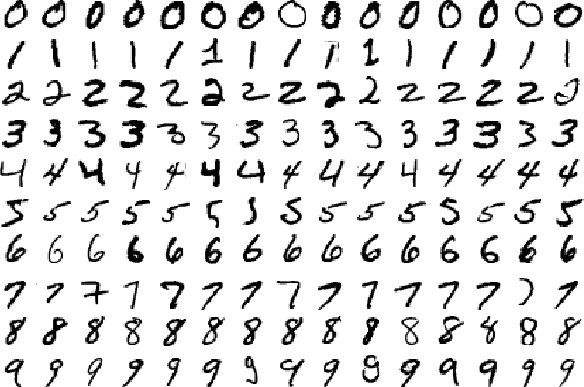
\includegraphics[scale=0.3]{img/mnist.jpeg}
	\end{minipage}
	\hfill
	\begin{minipage}{0.4\textwidth}
		\centering
		\caption{Exemplo notMNIST} 
		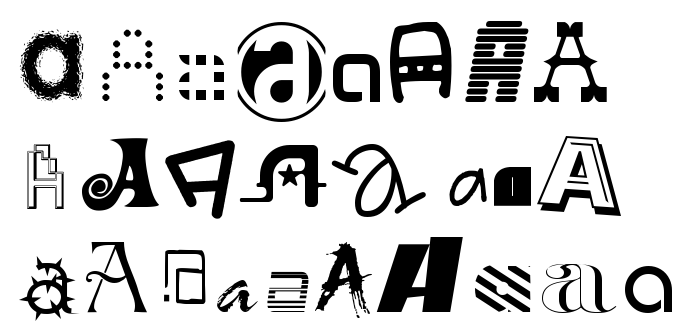
\includegraphics[scale=0.3]{img/nmn.png}
	\end{minipage}
\end{figure}

\begin{figure}[htb]
	\caption{Tradu��o de textos em imagens}
	\begin{center}
		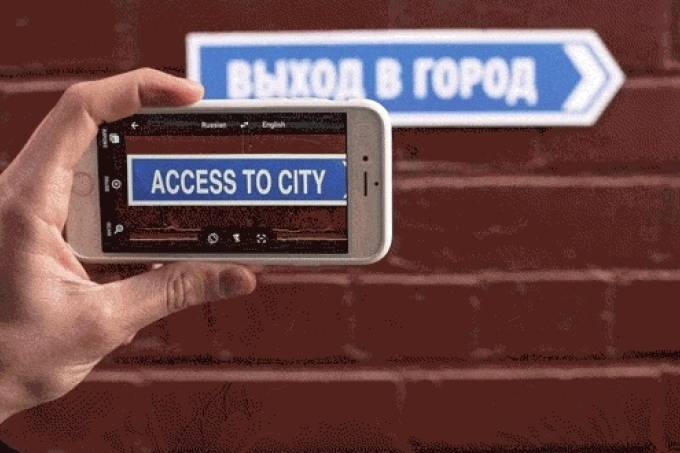
\includegraphics[scale=0.3]{img/google_tradutor.jpeg}
	\end{center}
\end{figure}


O desenvolvimento de bases de imagens para pesquisa s�o mais comuns no campo da medicina, motivados pelo desenvolvimento de tecnologias de apoio a disgn�sticos, como o projeto DMR - Database For Mastology Research (http://visual.ic.uff.br/dmi/) do Instituto de Computa��o da Universidade Federal Fluminense IC/UFF, que disponibiliza imagens mastol�gicas t�rmicas, mamografia, resson�ncia magn�tica e de ultrassom para a detec��o precoce do c�ncer de mama.


\subsection{Cataloga��o de dados}

Quando um pesquisador n�o tem dispon�vel uma fonte de dados que atenda a �rea de estudo de seu interesse, este precisa coletar as informa��es como parte de seu trabalho, para ent�o process�-las e concluir sua pesquisa.

A necessidade de cria��o de uma base de dados espec�fica, pode exigir uma grande coleta de amostras a campo em uma per�odo curto de tempo, com v�rias repeti��es, o que demandaria uma equipe e equipamentos, aumentando o tempo e o custo da pesquisa.

Em um cen�rio de pouco incentivo em pesquisa e curtos prazos na corrida por publica��o, alguns pesquisadores, ap�s investirem na cria��o de bases de informa��es adequadas para seus estudos, n�o facilitam o acesso dos dados para que outros possam pesquisar m�todos diferente, fato que poderiam gerar melhores resultados e aumentar o conhecimento cient�fico. Por outro lado, pesquisadores criam projetos que serviram de base para v�rios outros trabalhos, fomentando a tecnologia e o desenvolvimento do seu campos de pesquisa.

Este trabalho tem a miss�o de desenvolver uma fonte de dados ampla e confi�vel, para apoio a pesquisas em uma �rea importante para o agroneg�cio brasileiro: a produ��o de soja.

%a soja%
%A participação do Brasil na Produção Internacional%
%A importância da soja para o mercado financeiro e na indústria alimentícia%
%A importância da soja para o Brasil%
%Sobre o controle de produção%
%Sobre os laboratórios de sementes e os teste%
%Sobre o tetrazólio%


\section{A Soja}
A soja cultivada atualmente é muito diferente dos seus ancestrais, que eram plantas rasteiras que se desenvolviam na costa leste da Ásia, principalmente ao longo do rio Yangtse, na China.  Sua evolução começou com o aparecimento  de plantas oriundas de cruzamentos naturais entre duas espécies de soja selvagem que foram domesticadas e melhoradas por cientistas da antiga China.

Cultivada e consumida há milhares de anos pelas civilizações orientais, foi somente a partir do século vinte que foi comercialmente cultivada no Ocidente, mais precisamente nos Estados Unidos(EUA), a partir da década de 1920. Até 1940, a área de soja cultivada para forragem era maior que a cultivada para grãos. A partir de 1941, a área cultivada para grãos superou a cultivada para forragem. \cite{Amelio2011}

\subsection{A participação do Brasil na Produção Internacional}
Segundo \citeonline{FAS2018}, entre os anos de 19xx e 2017, o Brasil liderou a produção de soja no mundo ao lado dos EUA. Atualmente os dois países juntos são responsáveis por 66\% da produção mundial, com 114,10 e 116,92 milhões de toneladas métricas (mmt). A previsão da produção de soja para 2018/19 no Brasil, por \cite{FAS2018}, é um recorde de 117,0 milhões de toneladas métricas (mmt), em uma área colhida prevista para de 36,5 milhões de hectares (mha), 4\% em relação ao ano anterior, prevendo a produtividade de 3,21 toneladas por hectare, mantendo acima da média dos últimos cinco anos. 

\citeauthor{FAS2018} relata que o Brasil deverá continuar sendo o principal exportador de soja em 2018/19, impulsionados pela forte demanda global liderada pela China por alimentos proteicos, estimulando o esmagamento para obtenção do farelo o óleo de soja.

%ver \cite{Junior2017}

\subsection{A importância da soja para o mercado financeiro e na indústria alimentícia}
A commoditie de soja é negociada nas principais bolsas mundias e seu volume de negociações atualmente segundo (????) é de xxx bilhões de toneladas e yyy bilhões de dólares.\nota{Se este paragrafo for se manter, vou procurar os dados e fontes corretas} No Brasil e em vários países o valor da soja é usado para indexar contratos de diversas naturezas envolvendo o agronegócio, principalmente na compra de terras, maquinários agrícolas e empréstimos para financiamento da produção.

O grão de soja tem grande valor na economia global devido suas propriedades nutricionais e na produção de óleos
Usado na alimentação humana e animal a soja fornece grande quantidade de carboidratos e vitaminas, a proteína de soja é muito usada na indústria alimentícia e gastronômica como alternativa a proteína da carne e do leite, atendendo o mercado vegano e de restrições alimentares. A maior utilização da fibra alimentar da soja é na farinha de soja usada em raça animal, muito utilizada na produção de proteína animal, como carne bovina, suína e de frango.

O processo de beneficiamento da soja inclui a extração do óleo vegetal de soja, largamente usado na indústria alimentícia, sendo um dos mais acessíveis para o consumidor final. Segundo \cite{FAS2018a} o óleo de soja é o mais produzido e consumido no mundo entre as oleaginosas. 

\subsection{A importância da soja para o Brasil}
Para atingir tais grandezas de produção a cadeia agroindustrial da soja emprega certa de XXX pessoas no Brasil, e cerca de YYY empresas recolhendo aproximadamente XXX Milhões de reais em impostos, que representou zz\% da arrecadação do setor primário em 2017.\nota{Se este paragrafo for se manter, vou procurar os dados e fontes corretas}

O cultivo da soja no Brasil ao longo dos anos proporcionou a colonização de regiões pouco habitadas no interior do país, promovendo urbanização e crescimento econômico mais distribuído no território nacional. Entretanto cria um desafio para os produtores de soja, que encontram diferentes climas, biomas, solo, ciclos de chuvas e outros fatores, em um país de proporções continentais. Atualmente o Brasil possui registradas xxx cultivares diferentes de soja, sendo zz transgênicas cada cultivar tem suas características como variando a duração das etapas de produção, produção de óleo ou massa seca, quantidade e tamanho dos grãos, estrutura das plantas (tamanho da planta, raízes, volume de folhas), resistência a seca ou ao excesso de água, resistência a herbicidas, muitas variedades transgênicas são modificadas geneticamente para serem nocivas a determinados predadores, diminuindo o uso de inseticidas e fungicidas. Muita da tecnologia brasileira em sementes se origina da EMBRAPA, que atualmente possuem patentes de xxx cultivares de soja transgênica e zzz patentes de cruzamentos naturais.

ver \cite{Junior2017} \cite{LIMA2013} \nota{Material que comecei a ler e posso usar para embasar o texto}

\subsection{Sobre o controle de produção}
Devido a grande importância que a soja representa para nação brasileira é necessário que se proteja o processo de cultivo. Para isso o estado exige uma série de registros e controles sobre a produção, colheita, comercialização, transporte e exportação. Em cada etapa do processo produtivo da soja existem mecanismos de fiscalização por órgãos competentes.
A legislação Brasileira regula quais variedades de soja tem o cultivo permitido no Brasil, com o intuito de controlar a entrada de plantas que podem ser portas de entrada para fungos e insetos, que podem desequilibrar o ecossistema onde local. Situações como esta já aconteceram no Brasil em culturas de cacau, café e banana no passado, prejudicando a economia e o meio ambiente por vários anos

Para garantir autonomia e proteção dos custos de produção, os produtores de soja no Brasil podem produzir suas próprias sementes para safras futuras, mas se houver comercialização de sementes várias normas de qualidade devem ser seguidas, como por exemplo o teste de germinação que determina que se um lote de sementes não possuir o potencial de germinação mais que 70\% das sementes o lote é inviável para o plantio e deverá ser comercializado como grão no mercado secundário.

??? indica que uma produção inferior a 70\% de germinação é inviável em relação aos custos de produção, desta forma a utilização de lotes controlados aumentam as chances de sucesso na safra, diminuindo os riscos que as financiadoras de crédito e seguradoras rurais têm ao liberarem empréstimos aos produtores. Em 2017 xxx Milhões de reais foram liberados para produção de xx\%v das lavouras na Brasil.

\subsection{Sobre os laboratórios de sementes e os testes}
Até 2017 o Brasil possuem cerca de xx mil empresas e cooperativas que comercializam sementes de soja, sendo que xx\% possuem seus próprios laboratórios de análise de sementes, que realizam diversos testes de rotina, afim de determinar a qualidade e detectar as possíveis causas de problemas, para que estes sejam corrigidos. 

Além dos testes exigidos por lei, os testes oficiais de pureza e germinação, é comum as empresas fazer os testes de qualidade como (patologia  tetrazólio - Vigor - Envelhecimento Acelerado - Teste de emergência em areia - condutividade elétrica), para detectar patógenos e determinar inclusive se o processo de colheita e armazenagem foram feitos com qualidade ou causaram danos nas sementes e comprometeram o lote. Determinar a causa da inviabilidade de um lote é vital para ajustar o processo antes que mais lotes sejam comprometidos.

Os laboratórios de sementes empregam mais de x mil analistas no Brasil inteiro, e todo ano instituições como a EMBRAPA formam novas turmas de analistas para atenderem as demandas do mercado. O investimento que as empresas fazem com laboratório, analistas e equipamentos aumentam o custo da semente, mas agregam muito valor na qualidade e garantia das safras seguintes.

\subsection{Sobre o tetrazólio}
Uma das análises mais importantes de um laboratório de sementes de soja é o teste de \sigla{TZ}{Tetrazólio}, que a partir de uma amostra do lote de sementes, tem o objetivo de ressaltar os danos causados em cada semente, para que seja determinada em primeiro momento a viabilidade do lote e a vigorosidade que as plantas terão ao serem plantadas, e em segundo momento se houverem danos nas sementes, determinar o grau dos danos e as causas, que geralmente são causados por excesso de umidade no armazenamento, danos mecânicos do processo de colheita, secagem e estocagem; e danos causados por percevejos que se alimentam dos nutrientes contidos nas sementes.

Para realização do teste cada amostra é submetida a uma solução de sal de tetrazólio por até x horas, dependendo da metodologia usada, durante esta etapa a semente absorve a solução ficando maior e destacando em tons de vermelho carmim os danos que cada semente sofreu. Após a preparação inicial, cada semente é cortada no sentido transversal a radícula para análise do interior e exterior da mesma, na sequência é realizada uma minuciosa analise visual de cada metade da semente em busca de padrões característicos dos danos mencionados, os danos de cada semente são anotados em uma ficha de controle e ao final o analista calcula os resultados que classificam o lote.

As limitações do teste de tetrazólio, citadas por FRANÇA-NETO (1998) incluem a exigência de um treinamento especial sobre a estrutura embrionária da semente, experiência e paciência pois a análise é relativamente tediosa. Atualmente o mercado exige cada vez mais profissionais capacitados em realizar o teste.


Dada a importância que o teste de tetrazólio tem no processo de garantia de sucesso no cultivo da soja, e a importância da cadeia produtiva no Brasil e no mundo, é justificável que pesquisas sejam aplicadas com o objetivo de tornar o processo de análise mais rápido e assertivo.



%\section{Sobre o projeto}


%openCV android




\section{Flutter}


%%%%%%%%%%%%%%%%%%%

%%%%%%%%%%%%%%%%%%%

Eu vou estar indo sobre o b�sico de Dart, especialmente porque � usado por flutter e mais desenvolvimento de aplicativos ganhou muita tra��o ao longo dos anos e h� um monte de lucro a ser ganho.


Eu come�o falando sobre flutter e depois me movo para o dardo.



2. O que � Flutter?

Vamos come�ar com o primeiro take o que � flirter para aqueles de voc�s que talvez n�o conhe�am o Google Flirter como o nome indica � SDK de aplicativo m�vel do Google, que pode ser usado para criar interfaces nativas de alta qualidade em iOS e Android em um curto per�odo de tempo.

O lan�amento inicial do flirter foi em maio de 2017.

Tamb�m uma nota lateral SDK significa desenvolvimento de software.

Boa.

Voc� deve saber que o flirter faz uso do c�digo existente para funcionar.

Os muitos benef�cios oferecidos o levaram a ser usado por desenvolvedores de aplicativos independentes e at� por organiza��es famosas em todo o mundo.

Tamb�m � livre para usar uma fonte aberta.

Algumas das coisas b�sicas sobre o flerte que voc� deve tomar nota.

Nosso n�mero um desenvolvimento r�pido usando flirter.

Voc� pode ter recarregado em uma quantidade de milissegundos para garantir que seu aplicativo possa ganhar vida no menor tempo poss�vel.

Voc� tamb�m pode usar uma vasta gama de widgets totalmente personaliz�veis ??que ajudam a criar interfaces nativas da maneira mais r�pida poss�vel.

Eu estou falando de ser capaz de construir em minutos aqui.

N�mero dois interface expressiva e flex�vel s�o interface do usu�rio.

Seu aplicativo n�o pode ser bem-sucedido se n�o for f�cil de usar para as pessoas.

Os melhores aplicativos l� fora tamb�m apresentavam a melhor experi�ncia e a experi�ncia do usu�rio.

Ent�o, o que voc� conseguir mais ferramentas para garantir que o nativo e experi�ncia do usu�rio � o melhor que pode ser.

A arquitetura em camadas oferece acesso � personaliza��o completa, permitindo que voc� crie aplicativos interativos e amig�veis ??ao usu�rio, que t�m uma renderiza��o de renderiza��o incrivelmente r�pida, al�m de um expressivo desempenho nativo da �rvore de n�meros.

Independentemente de uma pessoa estar usando um dispositivo Android e iOS, seu aplicativo precisa oferecer a experi�ncia que eles esperam que os widgets no flertador possam incorporar todas as diferen�as cr�ticas de plataforma para garantir a qualidade.

Essas diferen�as negras incluem �cones de rolagem de navega��o e garfos para a incorpora��o do DS �s diferen�as. O desempenho nativo de seus aplicativos em dispositivos Android e iOS � mantido no n�vel ideal.

Agora que voc� adquiriu um conhecimento b�sico do Google Flirter, deixe-me dar uma r�pida introdu��o indireta ao escuro.



3 O que � o Dart?

O que � obscuro quando se trata de entender darte voc� deve saber que j� � um objeto e fez e florescer a linguagem definida que voc� usa a sintaxe no estilo C que compila opcionalmente no javascript d'arte oferece muito apoio.

Isso significa que ele pode suportar interfaces de classes abstratas que fazem sentido digita��o est�tica e at� mesmo um sistema de tipo de som.

Agora, todos esses termos podem soar um pouco demais para aqueles que n�o est�o familiarizados com esse jarg�o.

Bem, deixe-me tornar as coisas mais f�ceis para voc�.

Basicamente escuro ajuda voc� a criar lindas experi�ncias de alta qualidade em todas as telas de dispositivos por meio de uma linguagem que nega a otimiza��o de ferramentas flex�veis f�ceis de usar e de estruturas muito poderosas e ricas no pr�ximo cap�tulo.

Falarei sobre e levarei todos voc�s em um breve hist�rico de desenvolvimento de aplicativos para dispositivos m�veis, como evolu�ram ao longo dos tempos e por que voc�, como um poss�vel desenvolvedor da ABB, pode se tornar conhecido nesse campo por meio do Google furter ou talvez de algum outro SDK voc� est� confort�vel com o uso.

Ent�o vamos seguir em frente.


Se��o 2: A Hist�ria do Desenvolvimento de Aplicativos M�veis

4. Conhecendo seu hist�rico de aplicativos

Como mencionei, o desenvolvimento de aplicativos cresceu muito nos �ltimos anos.

Como algu�m que est� interessado em entrar nesse campo, ser� bom ter uma vis�o geral de como o mercado de desenvolvimento de aplicativos para dispositivos m�veis cresceu.

Quando eles foram introduzidos pela primeira vez, os telefones celulares foram completados como tecnologia que era usada apenas para fazer liga��es telef�nicas.

No entanto, mais tarde, como sabemos que o jogo mudar a inven��o de smartphones levou � abertura da porta de desenvolvimento de aplicativos m�veis, os aplicativos de software s�o como os chamamos de trabalho para lev�-los a executar ou operar em dispositivos m�veis modernos, como tablets e smartphones.

Com o passar dos anos, esses aplicativos foram aprimorados e agora parece ter se tornado uma parte importante de nossas vidas.

Eles parecem ter se integrado perfeitamente ao nosso estilo de vida, come�ando pelo in�cio do celular.

Vamos come�ar isso de todo o caminho de volta.

Sim, estou falando do come�o do celular e sim da primeira liga��o de celular feita.

Para aqueles de voc�s que n�o conhecem a primeira liga��o de celular j� feita, em 3 de abril de 1973, a mesma liga��o foi feita por Martin Cooper, da Motorola.

De fato, esse telefonema era basicamente um golpe de publicidade para a grande empresa.

N�o foi at� 10 anos depois, desde que a bola que o primeiro telefone celular atingiu oficialmente o mercado, mesmo assim, o jornal p�blico n�o foi capaz de us�-lo.

Por qu�.

Bem, porque a morte n�o � o primeiro telefone celular no mercado custou uma grana por \$ 2000 e pesava aproximadamente � 2.

Sim.

Isso � muito.

Agora, � claro, esse modelo inicial da Foon n�o tinha nenhum aplicativo.

Quero dizer, as pessoas provavelmente nem sabiam sobre apps naquela �poca, foi na d�cada de 1990, quando o BBH foi introduzido como os primeiros sistemas operacionais que permitiam aplicativos durante esse tempo espec�fico.

Esses dispositivos eram aqueles que inclu�am processadores de texto e bancos de dados de planilhas do di�rio.

� claro que a tecnologia melhorou e o TAAS BDA � um trabalho para se tornar acess�vel ao lidar com mais aplicativos.

Era uma linguagem de programa��o aberta que possibilitava aos usu�rios criar seus pr�prios aplicativos para o desenvolvimento de aplicativos personalizados.

As empresas precisam de dispositivos Foster e sim de sistemas operacionais ainda melhores.

Voc� pode n�o perceber isso agora, mas o lan�amento do smartphone BlackBerry, que n�o chegou l� em 2002, foi anunciado como uma grande conquista para as empresas de tecnologia.

Esse tipo de telefone foi capaz de integrar perfeitamente o email sem fio e outros recursos que foram os primeiros de muitos durante esse per�odo.

Java m e era muito popular para telefones e Beedi � por isso que voc� pode perguntar.

Isso porque permitia aos usu�rios espa�o adicional na mem�ria.

Ent�o, em 2009, o lan�amento do Symbian abriu as portas para novos desenvolvimentos ainda mais de acordo com os dados, pelo menos, 50 milh�es de dispositivos adotaram o sistema operacional Symbian depois que foi lan�ado.

Mesmo aparelhos da Nokia, aparelhos da Samsung e at� mesmo telefones LG come�aram a usar o novo sistema operacional para melhorar a si mesmos como marcas.

Ent�o, chegando ao desenvolvimento de aplicativos personalizados que atingiram o mainstream Bem, uma vez que os desenvolvedores come�aram o desenvolvimento come�ou a acelerar.

N�o demorou muito para que os apps atingissem o mainstream e o tempo do Grant.

Vivemos no.

N�s basicamente temos um aplicativo para cada tanque.

No entanto, voltando � hist�ria de tudo em 2007, o primeiro iPhone foi lan�ado pela Apple, a App Store foi adicionado pela empresa muito em seguida, permitindo aos usu�rios encontrar baixar e usar aplicativos.

No come�o, esses aplicativos eram limitados, mas n�o demorou muito para que os desenvolvedores de aplicativos descobrissem o potencial inexplorado nesse campo.

Seguindo o exemplo, o mercado Android deu �s pessoas uma outra plataforma para acessar aplicativos e at� hoje h� uma competi��o entre o aplicativo da Apple e do Android e eu acho que � para continuar.

E enquanto a competi��o entre o Android e a Apple continua e os desenvolvedores olham para as plataformas planas da base de clientes potenciais, forne�a-as.


Se��o 3: Por que usar o Flutter?
5. Entendendo por que voc� deve considerar o uso do Google
Flutter


Duvido que voc� conhe�a um pouco mais sobre o slurper e como ele pode ajudar voc� como desenvolvedor de aplicativos.

Vamos ver porque voc� deveria usar o Slichter.

Como mencionado antes, o flirter � o K Isso significa um kit de desenvolvimento de software.

� considerado por muitos como uma maneira eficiente de criar aplicativos m�veis de plataforma cruzada com uma interface de usu�rio ou interface do usu�rio impressionante.

Observe que a maneira desordenada de criar visualiza��es tem semelhan�as com o aplicativo da web.

� a� que voc� pode encontrar v�rias analogias para DML e CFS.

De acordo com os desenvolvedores do selector schlechter torna mais f�cil e r�pido para construir um belo aplicativo m�vel D-Wave flicker para a maioria das c�lulas.

Parece bom.

No entanto, para aqueles de voc�s que talvez n�o saibam sobre outras solu��es de plataforma cruzada, como Zahm nativo de re-a��o i�nica, voc� pode querer saber um pouco mais sobre como o Slichter pode ajudar.

Existem certos benef�cios ou o flerte Stec pode ajud�-lo a mudar de ideia.

E voc� sabe que voc� precisa come�ar a us�-lo.

Alguns de voc�s podem ter muitas perguntas sobre flertes agora.

Como funciona a carta?

Por que � considerado inovador pelos outros?

Por que eles deveriam us�-lo?

Etc ..

E espero responder a todos eles no discurso.

E embarque no benef�cio de o flicker ser o SDK im�vel para a cria��o de aplicativos m�veis de plataforma cruzada Krok � que voc� pode escrever um c�digo e depois executar o aplicativo no iOS e no Android.

O c�digo que voc� escreve tem que ser escrito no escuro.

Ent�o, qualquer idioma desenvolvido pelo Google Docs parecer� familiar para voc�.

Se voc� j� teve experi�ncia de usar Java antes.

Tome nota que, em vez de usar arquivos SML, voc� constr�i um layout.

Tal lay out � constru�do a partir de componentes de widgets que s�o aninhados seu widget � um aplicativo de material que � o aplicativo inteiro e, em seguida, voc� tem desconforto que � Dumaine lay out estrutura, em seguida, movendo-se dentro.

Voc� tem a barra de aplicativos que � como a barra de ferramentas do Android 2 e, em seguida, um cont�iner como o corpo.

Agora, � nesse corpo que voc� coloca os widgets layouts, como bot�es, texto, etc., avan�ando ou por que voc� deve considerar o uso do clicker. Veja uma lista.

N�mero um de recarga quente.

Como mencionado antes, o recarregamento do Hawks pode ser considerado como outro melhor recurso que � usado para recarregar.

Voc� pode criar instantaneamente os projetos em que est� trabalhando, como se estivesse construindo uma p�gina da Web, simplesmente alterando algo no c�digo.

Clique em carga de Hawtry e voc� poder� ver o resultado instantaneamente.

N�mero dois um conjunto inteiro de widgets de design de material que flertam voc� come�a a obter a ecosfera registrada com constru�do em componentes de interface do usu�rio, voc� deve tomar nota de que existem dois conjuntos de rejei��es.

H� o design do material que � para o Android e o Cupertino do Derrida, que � para iOS.

Voc� simplesmente tem que selecionar o widget que voc� quer e depois ir a partir da�.

Tamb�m n�o h� necessidade de voc� se preocupar com o fato de os widgets serem muito espec�ficos.

Isso significa que, mesmo que voc� acabe implementando alguns Cupertino, os widgets projetados por Maduna v�o acabar parecendo iguais em todos os dispositivos iOS e Android existentes.

Portanto, n�o h� necessidade de voc� se preocupar com algo em seu aplicativo ou at� mesmo com o aplicativo como um todo, parecendo diferente.

Quando executado em dispositivos diferentes No entanto, voc� pode usar diferentes equipes Android e iOS, se desejar.

Tamb�m tudo � um widget em flertar.

Sim, at� mesmo a sua classe de aplicativo, o aplicativo de material � um widget.

Ent�o, toda a sua estrutura de layouts � escaneada por dimens�o.

Ent�o, ter tudo como um widget permite que voc� use flirter para criar UI impressionante de uma maneira muito simples.

Numero tres.

V�rios pacotes, apesar de terem sido lan�ados mortos.

Recentemente, em 2007, a comunidade deflectiva de Dean � muito ativa e envolvida em torn�-la melhor.

Isso fez com que o flatter fosse capaz de suportar muitos pacotes que voc� tem acesso a pacotes para abrir imagens compartilhando a corrente e fazer solicita��es de HDTV acessando sensores armazenando suas prefer�ncias.

Implementando Firebase e a lista continua.

Todo esse suporte � para iOS e Android.

Agora que voc� passou por cima dos benef�cios do sluttier, pergunte a si mesmo. Voc� est� interessado em usar o flirter?

N�o h� necessidade de tomar uma decis�o precipitada.

Estarei falando mais sobre tudo isso enquanto o discurso continua.


Se��o 4: Como instalar o Flutter?
6. Instalando o Flutter para Windows, Linux e MacOS

N�mero um dos seus sistemas operacionais deve ser o Windows 7 S-B 1 s�o mais tarde de 64 bits, voc� precisa de pelo menos 400 M-B ou tr�s espa�o em disco.

Tome nota que n�o inclui este lugar para Dools.

Falando sobre as ferramentas que voc� precisa.

Ponto de shellfire Bovver.

Ou voc� n�o precisa.

Este � o G ID para o Windows.

Quando eles usam boa op��o de prompt de comando do Windows.

Se voc� tiver para o Windows j� est� instalado.

Precisa ter certeza de que voc� pode executar o comando get para o prompt de comando ou instalar o flirter no Mac

SO para instalar e executar o flirter no Mac OS, seu ambiente de desenvolvimento deve atender a esses requisitos m�nimos.

Estes s�o o sistema operacional deve ser, pelo menos, Mac OS 64 bits, pelo menos, 700 M-B de espa�o livre em disco.

Novamente, isso n�o inclui espa�o em disco para Dools.

Agora, observe que o flertador depende de v�rias ferramentas de linha de comando dispon�veis em seu ambiente.

Estes s�o Bash e Diyar r m.

Boa menina.

Descompacte e at� mesmo a �rvore num�rica.

Continuando a instalar o flirter no Linux para instalar e executar o flirter no Linux.

Voc� precisa de um sistema operacional que seja o Linux 64 bit 600 M-B de espa�o livre em disco.

Isso n�o inclui espa�o em disco para o seletor Dools, dependendo de algumas ferramentas de linha de comando dispon�veis

em seu ambiente.

Estes s�o novamente Bash e ganham Diyar.

R m.

Boa menina.

Descompacte e qual comando de teste flexor depende da biblioteca estar dispon�vel em seu ambiente que

� como voc� pode ver lib G.O. voc� Daut s o dot um fornecido por mim de bagagem, por exemplo l AB lib Glou one me no Ubuntu s�o Debian.

Voc� pode v�-lo no slide, ent�o n�o deixe de reservar o site oficial do seletor.

Voc� tem uma ideia mais aprofundada sobre o procedimento que precisa ser seguido para instalar e come�ar a usar o flexor.



Se��o 5: Benef�cios do Flutter
7. Benef�cios do Flutter

Com base em uma parte do Curso onde eu falei sobre o motivo pelo qual voc� deve considerar o uso do flirter um pouco mais sobre todos os benef�cios e pode oferecer a voc� muitos desenvolvedores recomendam usar o flirter.

Se voc� est� apenas come�ando no campo de desenvolvimento de aplicativos por causa de sua natureza amig�vel quando se trata de criar aplicativos multiplataforma, vamos passar por cima de uma lista.

Flirter de projeto de c�digo aberto n�mero um � um projeto de c�digo aberto que permite que ele esteja dispon�vel para uso tamb�m por startups.

Ele oferece muitas op��es para criar o tipo de aplicativo que voc� deseja criar para Android ou iOS.

Al�m disso, sendo de c�digo aberto, d� origem � colabora��o aberta, permitindo que outros ajudem a melhorar ou fa�a o n�mero dois de Ed impressionantes. integra��o usando flirter.

Voc� pode continuar e continuar adicionando e subtraindo edi��es durante o processo de desenvolvimento do aplicativo.

Oferece uma impressionante integra��o de edi��o com o est�dio Android e o c�digo do Visual Studio.

Isso leva a conclus�es mais inteligentes baseadas em onde os tipos de defini��es usuais e o n�mero de m�dulos importados criam campos escuros como o Java.

Por que a dieta diet�tica n�o � uma c�pia direta do Java.

Os dois s�o semelhantes a similaridades.

Ajude os desenvolvedores a mudar para o escuro.

Se eles est�o usando Java para o n�mero quatro da lista, temos 4 gerentes de engenharia que gerentes de engenharia tamb�m podem usar o flirter se tiverem a necessidade de liderar mais equipes de desenvolvimento biol�gico usando um SDK como gerente de engenharia.

Voc� pode criar uma equipe surda de um �nico aplicativo m�vel ou uma equipe de desenvolvimento para ajudar voc� a unificar os investimentos em desenvolvimento.

Voc� pode enviar recursos mais rapidamente para reduzir seus custos de manuten��o e transferir os mesmos recursos para o Android e o iOS simultaneamente.

Em suma, quando voc� est� usando a desordem, voc� tem acesso a melhores recursos de widgets f�ceis de usar e integra��es editoriais impressionantes para o desenvolvimento de aplicativos.

N�o � de admirar que muitos desenvolvedores tenham usado o seletor para criar aplicativos m�veis, mas tamb�m para alcan�ar um p�blico mais amplo.

No Android e no iOS.

Se��o 6: Quanta Experi�ncia como Desenvolvedor de Aplicativos
Devo ter que usar o Flutter?

8. Quanta experi�ncia como desenvolvedor de aplicativos eu deveria
tem que usar o Flutter?

Esta � a pergunta que muitos de voc�s podem ter atualmente.

Em suma, voc� n�o precisa de nenhuma experi�ncia anterior para aprender e usar flirter.

Este SDK � muito acess�vel para programadores que t�m uma ideia sobre conceitos de programa��o imperativa e conceitos orientados a objetos.

Contanto que voc� tenha paix�o e interesse em usar a desordem para criar aplicativos, voc� achar� o processo bastante f�cil e r�pido.

Vamos falar sobre isso um pouco mais.

N�mero um do estilo reativo ao usar o flirter, voc� precisar� come�ar em algum lugar para criar um aplicativo para iOS e Android.

� por isso que voc� precisa estar pronto para trabalhar usando uma estrutura reativa.

N�mero fazer.

David voc� n�o pode falar sobre seletor sem falar sobre a arquitetura de widgets que oferece.

Como mencionado tudo � o widget e seletor de seu elemento de estrutura para eles e voc� � o bot�o dois elemento muito estil�stico que voc� deseja usar, como um esquema de cores e formatar tudo.

� um isolante r�gido que permite criar o tipo de aplicativo que voc� quer sem problemas.

Voc� ganha muito controle sobre a renderiza��o do objeto de composi��o de execu��o do aplicativo e mais n�mero tr�s.

Diga adeus ao gerenciamento do ciclo de vida da atividade.

Se voc� � algu�m que se envolveu um pouco no desenvolvimento de aplicativos, voc� estar� familiarizado com o gerenciamento do ciclo de vida da atividade.

Ele s� aparece como trabalho extra, n�o �?

Uma atividade perif�rica, se poss�vel, que n�o seja adicionada diretamente no processo geral de produ��o de seu aplicativo.

No entanto, o que flertar voc� n�o ter� que se preocupar com o gerenciamento do ciclo de vida da atividade.

Isso ocorre porque o patch do conector de desordem ajuda a fazer com que todas as atividades transmitidas sejam vestidas e carregadas de maneira s�ncrona.

N�mero de 60 SPSS consistentes s�o quadros por segundo.

O Flirter tamb�m � �til para quem procura criar um seletor de aplicativos gr�ficos ou de jogos pesados, capaz de oferecer uma taxa consistente de 60 quadros por segundo devido � natureza reativa e ao uso de suporte sombrio.

Voc� ter� visuais est�veis ??em seu aplicativo desenvolvido.

O n�mero cinco, o flertador de suporte da comunidade, tamb�m tem uma grande comunidade de expedientes, al�m de demitir desenvolvedores que podem ajud�-lo com o suporte necess�rio que voc� precisa.

A comunidade torna mais f�cil para voc� aprender usando o flerte, bem como fazer conex�es �teis no campo de desenvolvimento de aplicativos.

Ent�o, vamos falar um pouco sobre darte e por que Slichter usa o come�o.

Se��o 7: Conhecendo o Dart
9. O que � o Dart e por que us�-lo?

Durante este curso eu mencionei d'arte muito como uma pequena atualiza��o.

Dart � uma linguagem de programa��o de uso geral que foi originalmente desenvolvida pelo Google.

Mais tarde foi aprovado como padr�o pela ECMA daks ECMA para 8 para ser mais preciso.

Voc� pode usar d'arte para construir aplica��es web e m�veis para servidores.

Ent�o, por que os desenvolvedores do d'arte trabalham no Google, al�m de outros.

N�o use darte para criar aplicativos de alta qualidade para iOS.

E Android, assim como a web.

Ent�o � por isso que pode ser visto ou � visto como uma �tima op��o quando se trabalha com recursos voltados para o desenvolvimento do lado do cliente.

Vamos a uma lista sobre o Bart.

A sintaxe escura produtiva n�mero um � clara e concisa.

O ferramental geral � muito simples, mas poderoso.

Voc� pode identificar erros sutis precocemente atrav�s da digita��o de sons usando darte.

Voc� tamb�m pode obter in�meras bibliotecas de pontua��o e milhares de pacotes.

N�mero dois r�pido Dart pode ser denominado como uma linguagem que oferece otimiza��o antes da viola��o.

Isso ajuda voc� a obter desempenho previsivelmente alto e inicializa��o r�pida em dispositivos m�veis e na Web.

O n�mero tr�s vi�vel para aplicativos m�veis escuros � executado de forma nativa no Android e no iOS.

Compiladores sombrios fazem A-R como um c�digo X 86.

Tome nota DEC para web app caiu spiles para javascript e � acess�vel.

Muitos desenvolvedores est�o familiarizados com o d'arte que voc� faz.

N�o � uma orienta��o e sintaxe de objeto sem surpresas.

Voc� pode facilmente pegar o jeito escuro se voc� j� sabe sobre Java s�o C ++.

Agora, se voc� sabe um pouco mais sobre d'arte Lexi, por que voc� deve considerar aprend�-lo em 2018, bem como por que o flerte faz uso do efeito.

Se��o 8: Por que voc� deve considerar o aprendizado de dardo em
2018

10. Se voc� considerar a aprendizagem do dardo em 2018 e
Al�m?

Se voc� tem pensado em aprender, aqui est� uma lista que pode ajud�-lo a tomar uma decis�o.

N�mero um f�cil de aprender.

Como mencionado anteriormente, os guardas de Daryn compartilham semelhan�as com outras linguagens comuns.

Isso tamb�m significa que voc� j� deve saber como usar d'arte sem perceber que ser� f�cil para voc� aprender se tiver experi�ncia com outras linguagens orientadas a objetos, como Java, s�o C ++.

Mesmo se voc� souber alguma aprendizagem sobre javascript, Darb n�o ser� dif�cil para voc�.

Outra grande coisa � que o dardo suporta tanto a digita��o solta quanto a forte.

Isso permite que seja mais f�cil quando voc� est� mudando de outro idioma.

Number faz uma base de c�digo compartilhada nativamente compilada.

Alguns de voc�s podem saber que outras estruturas permitem que voc� compartilhe partes da base de c�digo em diferentes plataformas.

No entanto escuro � um pouco diferente.

Ele permite que voc� escreva um �nico aplicativo que pode ser usado tanto no iOS quanto no Android, juntamente com a maneira como ele � compilado nativamente pelo Dubost.

Agora, � claro, isso � algo que os outros podem fazer, mas o darte � capaz de permitir ainda mais o compartilhamento.

Voc� sabe que eu posso dizer que permite que voc� compartilhe um pouco do seu c�digo entre a inteireza do seu GUI, n�o apenas os aplicativos m�veis fazem o Menke para diferentes plataformas, significando iOS e Android, mas tamb�m para a Web, bem como outras aplica��es de guarda tamb�m .

Isso permite que voc� compartilhe a maior parte do c�digo n�o UI ou digamos que o c�digo espec�fico em preto com o n�mero de frameworks do Underdark seja produtivo. Usando o escuro, voc� ter� a experi�ncia de como � f�cil e r�pido criar o layout e adicionar funcionalidade para o seu aplicativo.

Voc� pode criar o Caly no c�digo criando uma s�rie de widgets.

Lembre-se do que eu disse a voc� que, em flertar, tudo o que o widget usa com essas ferramentas certamente ajudar� voc� a criar o que quiser no menor tempo poss�vel.

N�mero quatro compila antes do tempo e apenas no tempo quando voc� est� desenvolvendo um aplicativo Avodart voc� pode ver as mudan�as que voc� faz instantaneamente.

Isso significa que voc� n�o ter� que passar pelo procedimento de recompila��o e n�o h� necessidade de esperar que o aplicativo seja recarregado.

Voc� s� precisa salvar a altera��o e ver instantaneamente as altera��es.

Isso � poss�vel porque, com essa estrutura de desenvolvimento de aplicativo para celular, voc� pode compilar antecipadamente.

R E ou D, bem como na hora certa.

R d.

Agora que voc� est� ciente das raz�es mencionadas, voc� provavelmente est� come�ando a entender o benef�cio de usar o darte.

Experimente e veja se � algo sobre o qual voc� deseja aprender mais.

Como um desenvolvedor de aplicativos que est� mudando meu discurso, eu deixo voc� saber por que flirter escolheu usar d'arte.

Se��o 9: Por que o Flutter usa Dart?

11. Por que o Flutter Decidiu Usar o Dart?
Flirter decidir usar d'arte n�o foi uma decis�o precipitada.

Flirter usa essa ferramenta.

Um total de quatro dimens�es prim�rias para avalia��o e considerou todas as necessidades dos autores, desenvolvedores e usu�rios finais do framework.

Foi fundada enquanto algumas l�nguas cumpriam certos requisitos.

Estava escuro l�.

Marcou muito em todas as dimens�es de avalia��o que foram verificadas pela equipe mais plana e tamb�m atendeu a todos os requisitos e crit�rios determinados.

Voc� deve saber que os dubladores de Darkthrone e compiladores suportam a combina��o de dois recursos cr�ticos para flertar um parding ao tema de flutter.

O primeiro � o ciclo de desenvolvimento r�pido baseado em GAAP, que permite a mudan�a de forma e a carga de Hawtry com estado na linguagem com tipos.

Como eu mencionei anteriormente, o GAAP est� na hora certa.

A segunda � a antecipa��o de nosso descompilador imenso, que emite uma importa��o A-R eficiente para uma inicializa��o r�pida e desempenho previs�vel de implementa��es de produ��o.

Al�m disso, a equipe de flirter foi capaz de trabalhar de perto com a comunidade DAR.

A comunidade � ativa e continua a investir recursos para melhorar o desenho quando se trata de us�-lo como exemplo.

Quando a equipe adotada darte decidiu definhar n�o teve uma hora antes do tempo ou toolbol AOB Freberg usando bin�rio nativo � um tal recurso � fundamental para alcan�ar alto desempenho previs�vel.

No entanto, agora a linguagem tem isso porque eles s�o dark deam e eles est�o construindo para Lucker no dia prim�rio um grande dia com dark marcou uma pontua��o alta para a vibra��o deam foram n�mero um produtividade do desenvolvedor de acordo com o tema.

Uma das principais proposi��es de valor de letras � que ele economiza recursos de engenharia, permitindo que desenvolvedores criem aplicativos para iOS e Android com a mesma base de c�digo usando uma linguagem altamente produtiva que acelera os desenvolvedores Forder e torna a carta mais atraente para eles.

Isso foi muito importante para a equipe de framework defletor da Dubow, bem como para os desenvolvedores.

Voc� deve saber que a maior parte da sorte � constru�da na mesma linguagem dada aos usu�rios.

Portanto, o tema precisa permanecer produtivo em cem mil linhas de c�digo sem sacrificar a acessibilidade ou a legibilidade da estrutura e dos widgets para os desenvolvedores.

Orienta��o n�mero dois objeto para flirter que vorn tema fez uma linguagem que foi adequado para flusters dom�nio do problema que � bom outra coisa que voc� vai usar suas experi�ncias de acordo com a equipe da ind�stria tem v�rias d�cadas de conveni�ncia construindo frameworks de interface do usu�rio em linguagens orientadas a objeto.

Embora eles possam ter usado uma linguagem conhecida orientada a objetos, isso significaria reinventar a roda para resolver v�rios problemas dif�ceis.

Al�m disso, a grande maioria dos desenvolvedores j� tem experi�ncia com desenvolvimento orientado a objetos, tornando mais f�cil aprender como desenvolver seus aplicativos, cujo seletor agora possui um alto desempenho previs�vel de acordo com o refletor de temas.

Eles querem capacitar os desenvolvedores para criar experi�ncias de usu�rio r�pidas e fluidas.

Ent�o, para que eles cumpram essa promessa ou objetivo, eles precisam ser capazes de executar uma quantidade significativa de placa de desenvolvedor durante cada quadro de anima��o.

Isso significa que a equipe precisava de uma linguagem que pudesse fornecer alto desempenho e fornecer desempenho previs�vel sem bater seus chefes.

Isso poderia causar o n�mero de quadros perdidos para localiza��o fasc neste ponto.

Voc� deve saber que a estrutura do defletor utiliza um fluxo de estilo funcional que, de acordo com o tema da letra, depende muito do eficiente alocador de mem�ria subjacente que manipula com efici�ncia o pequeno local de curta dura��o.

Este arquivo foi desenvolvido em linguagens com essa propriedade e n�o funciona de maneira eficiente em idiomas como esse recurso.

Ent�o agora voc� sabe por que flutter decidiu usar d'arte e por que voc� deveria estar familiarizado com tal linguagem.

E quem sabe voc� pode querer us�-lo tamb�m.


Se��o 10: Perguntas Freq�entes sobre o Flutter
12. O que h� dentro do Flutter SDK?
Permita-me ir com freq��ncia para fazer perguntas que voc� possa ter em mente que desapontam.

A primeira pergunta � o que est� dentro do SDK flertador.

Quando se trata de responder o que est� dentro do deflector SDK.

Aqui est� a lista.

O n�mero um otimizou fortemente o primeiro mecanismo de renderiza��o de leads duplo da Mumbai com excelente suporte para texto.

Em seguida, temos o conjunto de widgets de estilo de re-ato de Morgan o conjunto rico de widgets para Android e iOS que eu disse anteriormente tudo � um widget em flertar.

N�mero quatro, � bom para testes de unidade e integra��o.

Em seguida, entramos em interoperabilidade e plug-in API para conectar-se ao sistema e participar D DST gais headless best runner para executar testes em ferramentas de linha de comando do Windows Linux e Mac para criar testes de constru��o e compilar seus aplicativos.

13. O Flutter vem com uma estrutura?

Faz flutter vem com o quadro.

Sim.

Como desenvolvedores de aplicativos, voc� deve saber que os sistemas de terra plana com uma estrutura moderna inspirada pela estrutura de aletas de re-a��o foram projetados para serem lidos e personaliz�veis ??como um desenvolvedor.

Voc� pode ir em frente e optar por usar apenas parte do framework que voc� tem acesso, voc� � um framework completamente diferente.

A escolha � sua.


14. O Flutter vem com widgets?
Faz flutter vem com Vineyard como mencionado antes que sacode no parque e parte de flutter.

Ent�o, sim, selecione seus navios com um conjunto de alta qualidade McKeel design em layouts e equipes de widgets Cupertino.

Voc� tamb�m pode ir em frente e fazer seus pr�prios widgets ou at� mesmo personalizar qualquer um dos widgets existentes para criar o tipo de aplicativo que voc� deseja.

Novamente lembre-se tudo � um widget e flutter.


15. Como o Flutter roda meu c�digo no Android?

Como flertar meu no Android.

Alguns de voc�s podem estar se perguntando como o Slichter executa seu c�digo e o direito de lhe dar uma resposta simples.

De acordo com a equipe do flooder, o c�digo Engine C e C ++ s�o compilados com andr�ides e DK The Dark Lord.

Boada SDK do que o seu est� � frente do tempo.

AOP compilado em uma biblioteca ARMM nativa.

Essa biblioteca est� inclu�da em um projeto de corredor e dreich e a coisa toda � constru�da em qualquer B.K. quando � lan�ado, o aplicativo tende a carregar a biblioteca de defletores e qualquer renderiza��o na porta ou manipula��o de eventos, e assim por diante, s�o delegados ao c�digo do aplicativo e do flertador compilado.

Esse processo tamb�m � semelhante ao modo como muitos mecanismos de jogo funcionam e funcionam.


16. Como o Flutter executa meu c�digo no iOS?

Chegando a forma como o Echo � executado por flertadores em Io S de acordo com a equipe de niveladores, � muito semelhante a como ele � executado em um andr�ide.

O c�digo Engine C C ++ compilado com o LMM.

Mais uma vez, como mencionou o Lord das Trevas BODH, o SDK e o seu est�o � frente do tempo.

EO descompilado em uma biblioteca ARMM nativa.

Essa biblioteca est� inclu�da em um projeto runner Iowas e a coisa toda � constru�da em um ponto IPA quando lan�ada a biblioteca de defletores de carga de aplicativos e o mesmo processo de manipula��o de eventos de arte de importa��o de renderiza��o s�o delegados ao flirter compilado de um aplicativo chamado.


Se��o 11: Flutter o Futuro?
17. � Flutter o Futuro?

Depois de saber muito sobre flertar, faz sentido enganar Gwydir n�o s�o apenas cartas para o futuro.

Quando se trata de desenvolvimento de aplicativos Bem, vou tentar responder a esta pergunta de forma imparcial quanto poss�vel e, em seguida, schlechter Debbie est�o mortos.

Em 2007, Dean, a primeira vers�o est�vel do flirter, n�o ocorreu at� 9 de mar�o de 2018.

Ent�o voc� pode ver por si mesmo que ainda � muito cedo para chegar a uma defini��o ou uma decis�o definitiva sobre se o colecionador � ou n�o o futuro Arcand revolucionou o campo de desenvolvimento de aplicativos.

Um simples Layer Behrami determina sucesso flirter � ver se ele tem a capacidade de comparar o jogo bater nativo Riak estranho ou n�o.

Se voc� comparar os dois agora, ver� que re-age nativo atualmente tem a vantagem.

Se os dados sobre o flertador n�o servirem para nada, alguns usu�rios do iPhone X n�o consideram o flertador a melhor op��o para o desenvolvimento de aplicativos.

Al�m disso, re-showcase nativo apresenta in�meros aplicativos famosos, como Instagram Facebook Skype A B e B Wal-Mart e muito mais.

Al�m disso, alguns desenvolvedores acham que a biblioteca Cupertino ou Cupertino para iOS fornecida pelo flirter � muito limitadora em compara��o com os mais de 35 elementos da biblioteca de materiais.

Existem cerca de 14 componentes na biblioteca de Cupertino.

Talvez mais seja adicionado ao longo da linha.

Quem sabe.

Re-age nativo Por outro lado, tem muito a oferecer para iOS.

Agora, a cintila��o pode assumir a lideran�a quando se trata da interface do usu�rio.

Nossa implementa��o da interface do usu�rio.

Mas, novamente, � muito cedo para dizer algo sobre isso agora.

Vindo para proteger qual � a linguagem de programa��o subjacente usada por flertadores, n�o h� muita ado��o fora do Google.

� por isso que encontrar e contratar desenvolvedores daar capazes pode ser um problema para voc�.

Em compara��o com os desenvolvedores que usam especificamente desenvolvedores de javascript da d'Arte Borth-los em um n�mero de profissionais que voc� ser� capaz de encontrar apenas em 2018.

Dito tudo isso flirter tem alguns pontos fortes que est� atraindo mais usu�rios para o trabalho n�mero um escuro passa a ser mais r�pido do que o script java e no Slichter escuro Gordis compilado diretamente para o n�mero de tribunal ARMM voc� obter grande documenta��o para abart.

Al�m disso, os focos mais escuros s�o totalmente customizados, e os olhos s�o interfaces de usu�rio, o que � algo �timo, o que � �timo para aplicativos de marca.

A �ltima coisa � flutter � chamada de equipe de desenvolvimento de placa continuar trabalhando para torn�-lo melhor em vez de deixar tudo para a comunidade.

Ent�o, se voc� � algu�m que est� interessado em checar flirter, voc� definitivamente deveria.

Embora seja muito cedo para julgar se a talhadeira se tornar� ou n�o a pr�xima grande novidade no mundo do desenvolvimento de aplicativos.

Ele oferece muitos benef�cios que podem ajudar voc� a criar seu aplicativo economizando tempo.

Se��o 12: Google Flutter - Escolha seu caminho

18. Introdu��o - Google Flutter - Escolha seu caminho

Nesta parte do curso eu irei discutir se voc� deve ou n�o optar por um flerte na esperan�a de fazer uma carreira com ele e n�s estaremos indo para as op��es de freelancer, bem como as outras poss�veis vagas oferecidas pelas ind�strias que procuram para indiv�duos proficientes no Google Slichter e darte.

Ent�o vamos come�ar.


19. Flutter pode levar a uma carreira para voc�?

Como mencionado anteriormente na se��o sobre flutter � o futuro, o Google Slichter � relativamente novo e � por isso que apesar de oferecer muitos benef�cios aos desenvolvedores de aplicativos, ainda h� alguma hesita��o em selecion�-lo como um grande SDK para fazer uma carreira.

No entanto, existem todas essas exce��es � norma e h� profissionais prov�veis ??por a� que est�o experimentando um crescimento de carreira impressionante por causa de sua expertise em rela��o ao Google Flicker.

A resposta para essa pergunta depende de voc�.

Voc� faz ser relativamente novo.

N�o h� muitas vagas de emprego especificamente para pessoas que conhecem o Google Flirter.

� por isso que cabe a voc� decidir se deseja optar pela rota de freelancer para testar as �guas se quiser candidatar-se a uma posi��o em algum neg�cio.

Mais especificamente, se voc� quiser seguir em frente e trabalhar para o Google.

20. Freelancing como um desenvolvedor Flutter?

Come�ando com as op��es de freelancer que voc� pode aproveitar como um desenvolvedor de seletor e em um sentido relacionado algu�m que sabe darte o dinheiro que voc� ser� capaz de fazer depende do tipo de projeto que voc� ser� contratado para.

Principalmente as pessoas est�o procurando por desenvolvedores de vibra��es porque querem contratar algu�m para ajud�-los a criar um aplicativo.

Tais trabalhos geralmente incluem tudo diferente e tamb�m um rosto de costas e desenvolvimento.

Voc� pode at� mesmo ter que debater com a pessoa que o contratou para polir o aplicativo at� o pagamento de um �nico projeto, dependendo do que isso implica.

Pode variar de \$ 200 a t�o alto quanto Dan.

Mil d�lares.

E estou falando da moeda norte-americana.

Nem um monte de gente se mudou para fliter.

No entanto, � prov�vel que, com o tempo, mais pessoas optem pelo flerte, o que dar� origem a empregos com sal�rios mais altos para os desenvolvedores de flertes.


21. Sites para encontrar trabalho como um desenvolvedor Flutter

Humana, v� para a seguinte lista de sites que oferecem trabalho, o tipo de trabalho que voc� ser� capaz de obter depender� de sua experi�ncia e conjunto de habilidades.

Os sites da Web s�o para trabalhos de Lance.

Pro blogger eu freelance 99 projeta o projeto criativo grope guru para contratar.

� claro que existem mais sites que podem oferecer a voc� o trabalho como desenvolvedor de flirter.

Ent�o tudo que voc� precisa fazer � pesquisar sobre eles on-line e ver qual site funciona melhor para voc�.


22. Trabalhando com um neg�cio como um desenvolvedor indecente

Se voc� deseja ser contratado por um neg�cio como um desenvolvedor flutuante, ent�o h� alguns que podem contrat�-lo.

O Google � sua melhor op��o se voc� tiver experi�ncia em schlechter.

Voc� pode acabar sendo contratado pelo Google como gerente de programa t�cnico.

As responsabilidades de tal trabalho incluem o gerenciamento de programas de programas t�cnicos e projetos que trabalham em estreita colabora��o com engenheiros e pessoal t�cnico para desenvolver e acompanhar marcos e cronogramas de libera��o para muitas pe�as m�veis que precisam se unir.

Desenvolver um plano e cronograma com marcos bem definidos gerenciando a comunica��o do progresso e atualiza��es de status dentro do n�cleo e estender as equipes significando o cliente e parceiros e escalar os problemas conforme necess�rio, avaliando a qualidade de resiste ao monitoramento real de bugs e altera��es de acordes para identificar problemas de qualidade e tend�ncias no desenvolvimento de ferramentas e processos para melhorar a produtividade da engenharia de software de acordo com os dados atuais.

O sal�rio m�dio nacional de um gerente de programa t�cnico s�nior nos Estados Unidos �.

Espere por uma �rvore 8 0 6 9 d�lares, ent�o isso � como uma centena.

Mais de 100.000 d�lares americanos anualmente no desenvolvedor sluttier.

Voc� tamb�m pode ser contratado por empresas como desenvolvedor de software.

Enquanto o pagamento para os desenvolvedores de software pode variar de noventa mil d�lares fazer um pouco mais de mil d�lares por ano.

O espa�o do desenvolvedor de software deve aumentar 22% de 2012 para 2022, o que pode ser uma boa op��o para voc� como profiss�o.


23. Habilidades b�sicas para ter como um desenvolvedor Flutter

Se voc� est� pensando em come�ar sua carreira como desenvolvedor de flirter, voc� deve saber sobre certas habilidades b�sicas.

Estas habilidades recomendadas s�o voc� deve saber como renderizar uma tela usando aplicativos Mondial seguido de uma barra de ma��.

Voc� deve saber como definir o porqu� de uma coluna e linha voc� deve saber como usar o recipiente para tatear e conte�do um palpite.

Voc� deve saber o uso de texto e imagem e como eles podem ser usados ??em conjunto.

Voc� deve conhecer o funcionamento da imagem do ativo e da imagem da rede.

Voc� deve ser criativo e �nico com suas ideias.

Voc� deve ser capaz de trabalhar em tarefas individuais, bem como projetos de grupo.

Voc� deve ser capaz de liderar uma equipe de desenvolvedores, se necess�rio.

Voc� deve ser capaz de personalizar o aplicativo que um churrasco declina os requisitos.

Voc� deve ter conhecimento e saber como funciona o dardo porque eu mencionei as pontua��es que voc� precisa saber sobre o escuro.

Se voc� pretende usar o Google sluttier voc� deve ser capaz de usar o detector de Jester para fazer bot�es flex�veis e personalizar.

Voc� deve ter uma boa comunica��o com as habilidades de Anderton.

Como eu disse, essa � uma lista de habilidades recomendadas, mesmo que voc� n�o conhe�a essas habilidades agora, pode aprender com expedientes ao entrar em campo e continuar sua jornada como desenvolvedor do seletor do Google.

24. Usando M�dias Sociais para Encontrar Empregos como um Desenvolvedor Flutter


Usando a m�dia social � outra maneira para voc� possivelmente ser contratado como um desenvolvedor de flirter para tratar plataformas de m�dia social.

Voc� pode usar est�o ligados e esta � uma plataforma maravilhosa para encontrar empregos.

Voc� s� precisa fazer o login ou se inscrever se ainda n�o tiver uma conta.

Em seguida, fa�a o seu perfil e comece a acompanhar a empresa do que as pessoas que voc� conhece bem aquecidas ou est�o contratando desenvolvedores flirter, certificando-se de que seu perfil esteja atualizado.

� embarcar quando voc� est� usando vinculado e porque os potenciais empregadores podem v�-lo se eles s�o como o que voc� tem para oferecer.

Eles podem voltar para voc� sobre o trabalho no Facebook.

O Facebook � uma plataforma de m�dia social popular.

Ele permite que as pessoas se conectem umas com as outras de todo o mundo, portanto, usam essa plataforma e come�am a desenvolver contatos.

Voc� pode participar de grupos e p�ginas que permitem que voc� se conecte com pessoas e empresas que est�o procurando contratar pessoas para o trabalho, bem como dependendo das pontua��es.

Como desenvolvedores Twitter flertam Twitter para Twitter voc� pode acompanhar empresas e pessoas no campo de futebol do Google para ver se eles est�o contratando.

Voc� tamb�m pode iniciar uma conversa com desenvolvedores influentes respondendo aos tweets deles e criando o relat�rio para ajud�-lo em sua carreira.


25. Dicas de Cria��o de CV

Seja um desenvolvedor flittered bem sucedido � crucial que voc� d� o primeiro passo certo.

E esse � o seu curr�culo.

Mantenha o seu CV espec�fico e ao ponto n�o adicione detalhes que n�o s�o �teis, mas tamb�m n�o se esque�a de adicionar informa��es relevantes.

Tenha em mente que algumas empresas t�m curr�culos espec�ficos para o Max que eles pedem que voc� siga quando estiver se candidatando a um emprego em suas empresas.

Eles podem diferir quando comparados a um CV padr�o, no sentido de que eles podem lhe fazer apenas algumas perguntas relevantes relativas ao trabalho de desenvolvedor de flirter e nada mais.

Algumas dicas CV incluem, em seguida, promover-se como um desenvolvedor flutuante.

� importante destacar sua experi�ncia at� mesmo volunt�ria.

Tente e evite chav�es s�o termos que parecem um exagero.

Tente apresentar sua experi�ncia e o que voc� pode trazer para a mesa sem usar palavras como incr�vel, realmente espetacular, altamente criativo, etc.

Voc� recebe um segundo par de olhos para ler seu curr�culo.

�s vezes, um novo par de olhos far� isso como um membro da fam�lia ou um colega de trabalho que voc� vestiu ou at� mesmo um amigo pode ajud�-lo a desencadear certos erros.

Antes de prosseguir, envie seu curr�culo.


26. Outras dicas para ajud�-lo como um desenvolvedor Flutter

H� muitas dicas que n�o o ajudaram em sua jornada como desenvolvedor de flertadores.

Alguns deles demoram o tempo necess�rio para fazer qualquer abertura de trabalho em potencial que esteja dispon�vel como desenvolvedor de flirter.

Voc� deve trabalhar com �tica e com total compromisso com o seu trabalho para construir uma boa reputa��o para si mesmo neste campo.

Como freelancer, voc� pode contratar um profissional de servi�os de contabilidade, mas manter o controle de seus registros e transa��es manter dados de backup para todas as suas transa��es.

N�o exagere quando voc� come�ar a trabalhar com widgets.

As vezes menos � mais.

Aprenda gradualmente conjunto de metas e objetivos para si mesmo que podem motiv�-lo.

Compartilhe seu trabalho com outras pessoas em quem voc� confia para obter cr�ticas construtivas.

N�o se afaste da ajuda e, mais importante, conhe�a a sua ala.


27. Freelancing ou uma contrata��o regular como um desenvolvedor Flutter?

Ent�o voc� deve optar por freelancer ou contratar uma perna regular como um desenvolvedor flutuante.

Bem, eu n�o tenho todas as respostas.

O que eu posso fazer � tentar gui�-lo apresentando os fatos para que voc� possa fazer a sua pr�pria mente.

Como eu mencionei ao longo do discurso, o Google Strutter � relativamente novo e levar� tempo para determinar se ele pode manter a posi��o contra um famoso caso de SD.

Se voc� � algu�m que est� interessado em aprender mais sobre flertes e voc� � apaixonado por isso, voc� deveria.

Saber usar flirter � uma boa habilidade para ter como desenvolvedor de aplicativos.

Talvez tente se concentrar mais no fogo.

Java JavaScript C ++ e half d'arte como uma ferramenta opcional para usar no futuro.

Se voc� � algu�m que sabe um pouco sobre iletrado e darte talvez lidar com um ou dois shows freelancer e ver como isso acabou por voc�.

Se voc� gosta de experi�ncia, ent�o talvez voc� possa se candidatar a uma posi��o em uma grande empresa.

Tamb�m secar um est�gio de flutter darte em uma empresa local tamb�m pode ajud�-lo a tomar uma decis�o final.

Se voc� deseja continuar como uma carreira novamente.

No final, tudo depende do que voc� deseja alcan�ar como desenvolvedor de aplicativos.

Quais idiomas e s DKs voc� acha prefer�vel usar e quanto dinheiro deseja fazer em sua carreira profissional.


Se��o 13: Resumo e Conclus�o
28. Resumo e Conclus�o

Muito obrigado por me acompanhar para discursar Espero que eu tenha sido capaz de lhe oferecer as informa��es que voc� precisava sobre o Slackware e a arte e se � ou n�o algo sobre o qual voc� deseja aprender mais.

Como um resumo r�pido, a Fluker foi criada pelo Google para oferecer aos desenvolvedores atrav�s do Platform SDK que n�o s� economiza tempo, mas tamb�m oferece v�rios recursos que voc� pode usar para criar aplicativos que sejam reativos e oferecidos e que a conveni�ncia do usu�rio seja eficiente.

Recomenda-se como uma boa op��o para os desenvolvedores que desejam criar aplicativos de jogos, outros aplicativos que s�o ricos em gr�ficos novamente.

Embora seja muito cedo para julgar se o flerte � a pr�xima grande coisa, o fato que n�o pode ser negado � que ele forneceu a v�rios desenvolvedores uma maneira mais f�cil de criar os aplicativos que eles desejam.

Ent�o, se voc� est� interessado em flertar e darte, eu recomendo aprender mais sobre isso.

Quem sabe voc� pode acabar gostando.

Tem para te oferecer.

Ent�o, novamente, muito obrigado por tomar o tempo para discursar comigo.

Fique aben�oado.







\nota{Aqui preciso colocar os trabalhos que já encontrei sobre análise de tetrazólio por imagem}

Ao constatar a importância que o teste de tetrazólio tem no processo de qualidade das sementes, e o impacto que gera na produção de soja no Brasil, é importante pensarmos em como a computação pode auxiliar no processo de analise de sementes no teste de tetrazólio.

.

.



Tetrazolio - Soja e outros \nota{Aqui que apresentar alguns trabalhos com tretazólio em soja e também em outras sementes, mostrado que outras culturas podem ser exploradas futuramente.}

.


.



Alguns trabalhos foram propostos na ultima década, com a intenção de usar visão computacional no auxilio da identificação dos danos de soja no teste de tetrazólio \nota{quero apresentar aqui os trabalhos que desenvolveram algum software específico para análise de tetrazólio e os métodos utilizados}


como \citeauthor{Rocha2016} usando o método de ....;\\
BBB usando o método de ....\\
CCC usando o método ...
	
.


.




Assim como \cite{Wendt2014, Junior2017} ... \nota{Apresentar trabalhos que usaram softwares genéricos de análise de imagem }


.

.



{\small \textst{escrever sobre base de dados para pesquisa }} \\

.




%processamento de imagens 

%deep learn

%{\small \textst{Uso de software não especifico}} \\

\section{a}

Assim como \cite{Wendt2014, Junior2017}



%

\section{Flutter}


%%%%%%%%%%%%%%%%%%%

%%%%%%%%%%%%%%%%%%%

Eu vou estar indo sobre o b�sico de Dart, especialmente porque � usado por flutter e mais desenvolvimento de aplicativos ganhou muita tra��o ao longo dos anos e h� um monte de lucro a ser ganho.


Eu come�o falando sobre flutter e depois me movo para o dardo.



2. O que � Flutter?

Vamos come�ar com o primeiro take o que � flirter para aqueles de voc�s que talvez n�o conhe�am o Google Flirter como o nome indica � SDK de aplicativo m�vel do Google, que pode ser usado para criar interfaces nativas de alta qualidade em iOS e Android em um curto per�odo de tempo.

O lan�amento inicial do flirter foi em maio de 2017.

Tamb�m uma nota lateral SDK significa desenvolvimento de software.

Boa.

Voc� deve saber que o flirter faz uso do c�digo existente para funcionar.

Os muitos benef�cios oferecidos o levaram a ser usado por desenvolvedores de aplicativos independentes e at� por organiza��es famosas em todo o mundo.

Tamb�m � livre para usar uma fonte aberta.

Algumas das coisas b�sicas sobre o flerte que voc� deve tomar nota.

Nosso n�mero um desenvolvimento r�pido usando flirter.

Voc� pode ter recarregado em uma quantidade de milissegundos para garantir que seu aplicativo possa ganhar vida no menor tempo poss�vel.

Voc� tamb�m pode usar uma vasta gama de widgets totalmente personaliz�veis ??que ajudam a criar interfaces nativas da maneira mais r�pida poss�vel.

Eu estou falando de ser capaz de construir em minutos aqui.

N�mero dois interface expressiva e flex�vel s�o interface do usu�rio.

Seu aplicativo n�o pode ser bem-sucedido se n�o for f�cil de usar para as pessoas.

Os melhores aplicativos l� fora tamb�m apresentavam a melhor experi�ncia e a experi�ncia do usu�rio.

Ent�o, o que voc� conseguir mais ferramentas para garantir que o nativo e experi�ncia do usu�rio � o melhor que pode ser.

A arquitetura em camadas oferece acesso � personaliza��o completa, permitindo que voc� crie aplicativos interativos e amig�veis ??ao usu�rio, que t�m uma renderiza��o de renderiza��o incrivelmente r�pida, al�m de um expressivo desempenho nativo da �rvore de n�meros.

Independentemente de uma pessoa estar usando um dispositivo Android e iOS, seu aplicativo precisa oferecer a experi�ncia que eles esperam que os widgets no flertador possam incorporar todas as diferen�as cr�ticas de plataforma para garantir a qualidade.

Essas diferen�as negras incluem �cones de rolagem de navega��o e garfos para a incorpora��o do DS �s diferen�as. O desempenho nativo de seus aplicativos em dispositivos Android e iOS � mantido no n�vel ideal.

Agora que voc� adquiriu um conhecimento b�sico do Google Flirter, deixe-me dar uma r�pida introdu��o indireta ao escuro.



3 O que � o Dart?

O que � obscuro quando se trata de entender darte voc� deve saber que j� � um objeto e fez e florescer a linguagem definida que voc� usa a sintaxe no estilo C que compila opcionalmente no javascript d'arte oferece muito apoio.

Isso significa que ele pode suportar interfaces de classes abstratas que fazem sentido digita��o est�tica e at� mesmo um sistema de tipo de som.

Agora, todos esses termos podem soar um pouco demais para aqueles que n�o est�o familiarizados com esse jarg�o.

Bem, deixe-me tornar as coisas mais f�ceis para voc�.

Basicamente escuro ajuda voc� a criar lindas experi�ncias de alta qualidade em todas as telas de dispositivos por meio de uma linguagem que nega a otimiza��o de ferramentas flex�veis f�ceis de usar e de estruturas muito poderosas e ricas no pr�ximo cap�tulo.

Falarei sobre e levarei todos voc�s em um breve hist�rico de desenvolvimento de aplicativos para dispositivos m�veis, como evolu�ram ao longo dos tempos e por que voc�, como um poss�vel desenvolvedor da ABB, pode se tornar conhecido nesse campo por meio do Google furter ou talvez de algum outro SDK voc� est� confort�vel com o uso.

Ent�o vamos seguir em frente.


Se��o 2: A Hist�ria do Desenvolvimento de Aplicativos M�veis

4. Conhecendo seu hist�rico de aplicativos

Como mencionei, o desenvolvimento de aplicativos cresceu muito nos �ltimos anos.

Como algu�m que est� interessado em entrar nesse campo, ser� bom ter uma vis�o geral de como o mercado de desenvolvimento de aplicativos para dispositivos m�veis cresceu.

Quando eles foram introduzidos pela primeira vez, os telefones celulares foram completados como tecnologia que era usada apenas para fazer liga��es telef�nicas.

No entanto, mais tarde, como sabemos que o jogo mudar a inven��o de smartphones levou � abertura da porta de desenvolvimento de aplicativos m�veis, os aplicativos de software s�o como os chamamos de trabalho para lev�-los a executar ou operar em dispositivos m�veis modernos, como tablets e smartphones.

Com o passar dos anos, esses aplicativos foram aprimorados e agora parece ter se tornado uma parte importante de nossas vidas.

Eles parecem ter se integrado perfeitamente ao nosso estilo de vida, come�ando pelo in�cio do celular.

Vamos come�ar isso de todo o caminho de volta.

Sim, estou falando do come�o do celular e sim da primeira liga��o de celular feita.

Para aqueles de voc�s que n�o conhecem a primeira liga��o de celular j� feita, em 3 de abril de 1973, a mesma liga��o foi feita por Martin Cooper, da Motorola.

De fato, esse telefonema era basicamente um golpe de publicidade para a grande empresa.

N�o foi at� 10 anos depois, desde que a bola que o primeiro telefone celular atingiu oficialmente o mercado, mesmo assim, o jornal p�blico n�o foi capaz de us�-lo.

Por qu�.

Bem, porque a morte n�o � o primeiro telefone celular no mercado custou uma grana por \$ 2000 e pesava aproximadamente � 2.

Sim.

Isso � muito.

Agora, � claro, esse modelo inicial da Foon n�o tinha nenhum aplicativo.

Quero dizer, as pessoas provavelmente nem sabiam sobre apps naquela �poca, foi na d�cada de 1990, quando o BBH foi introduzido como os primeiros sistemas operacionais que permitiam aplicativos durante esse tempo espec�fico.

Esses dispositivos eram aqueles que inclu�am processadores de texto e bancos de dados de planilhas do di�rio.

� claro que a tecnologia melhorou e o TAAS BDA � um trabalho para se tornar acess�vel ao lidar com mais aplicativos.

Era uma linguagem de programa��o aberta que possibilitava aos usu�rios criar seus pr�prios aplicativos para o desenvolvimento de aplicativos personalizados.

As empresas precisam de dispositivos Foster e sim de sistemas operacionais ainda melhores.

Voc� pode n�o perceber isso agora, mas o lan�amento do smartphone BlackBerry, que n�o chegou l� em 2002, foi anunciado como uma grande conquista para as empresas de tecnologia.

Esse tipo de telefone foi capaz de integrar perfeitamente o email sem fio e outros recursos que foram os primeiros de muitos durante esse per�odo.

Java m e era muito popular para telefones e Beedi � por isso que voc� pode perguntar.

Isso porque permitia aos usu�rios espa�o adicional na mem�ria.

Ent�o, em 2009, o lan�amento do Symbian abriu as portas para novos desenvolvimentos ainda mais de acordo com os dados, pelo menos, 50 milh�es de dispositivos adotaram o sistema operacional Symbian depois que foi lan�ado.

Mesmo aparelhos da Nokia, aparelhos da Samsung e at� mesmo telefones LG come�aram a usar o novo sistema operacional para melhorar a si mesmos como marcas.

Ent�o, chegando ao desenvolvimento de aplicativos personalizados que atingiram o mainstream Bem, uma vez que os desenvolvedores come�aram o desenvolvimento come�ou a acelerar.

N�o demorou muito para que os apps atingissem o mainstream e o tempo do Grant.

Vivemos no.

N�s basicamente temos um aplicativo para cada tanque.

No entanto, voltando � hist�ria de tudo em 2007, o primeiro iPhone foi lan�ado pela Apple, a App Store foi adicionado pela empresa muito em seguida, permitindo aos usu�rios encontrar baixar e usar aplicativos.

No come�o, esses aplicativos eram limitados, mas n�o demorou muito para que os desenvolvedores de aplicativos descobrissem o potencial inexplorado nesse campo.

Seguindo o exemplo, o mercado Android deu �s pessoas uma outra plataforma para acessar aplicativos e at� hoje h� uma competi��o entre o aplicativo da Apple e do Android e eu acho que � para continuar.

E enquanto a competi��o entre o Android e a Apple continua e os desenvolvedores olham para as plataformas planas da base de clientes potenciais, forne�a-as.


Se��o 3: Por que usar o Flutter?
5. Entendendo por que voc� deve considerar o uso do Google
Flutter


Duvido que voc� conhe�a um pouco mais sobre o slurper e como ele pode ajudar voc� como desenvolvedor de aplicativos.

Vamos ver porque voc� deveria usar o Slichter.

Como mencionado antes, o flirter � o K Isso significa um kit de desenvolvimento de software.

� considerado por muitos como uma maneira eficiente de criar aplicativos m�veis de plataforma cruzada com uma interface de usu�rio ou interface do usu�rio impressionante.

Observe que a maneira desordenada de criar visualiza��es tem semelhan�as com o aplicativo da web.

� a� que voc� pode encontrar v�rias analogias para DML e CFS.

De acordo com os desenvolvedores do selector schlechter torna mais f�cil e r�pido para construir um belo aplicativo m�vel D-Wave flicker para a maioria das c�lulas.

Parece bom.

No entanto, para aqueles de voc�s que talvez n�o saibam sobre outras solu��es de plataforma cruzada, como Zahm nativo de re-a��o i�nica, voc� pode querer saber um pouco mais sobre como o Slichter pode ajudar.

Existem certos benef�cios ou o flerte Stec pode ajud�-lo a mudar de ideia.

E voc� sabe que voc� precisa come�ar a us�-lo.

Alguns de voc�s podem ter muitas perguntas sobre flertes agora.

Como funciona a carta?

Por que � considerado inovador pelos outros?

Por que eles deveriam us�-lo?

Etc ..

E espero responder a todos eles no discurso.

E embarque no benef�cio de o flicker ser o SDK im�vel para a cria��o de aplicativos m�veis de plataforma cruzada Krok � que voc� pode escrever um c�digo e depois executar o aplicativo no iOS e no Android.

O c�digo que voc� escreve tem que ser escrito no escuro.

Ent�o, qualquer idioma desenvolvido pelo Google Docs parecer� familiar para voc�.

Se voc� j� teve experi�ncia de usar Java antes.

Tome nota que, em vez de usar arquivos SML, voc� constr�i um layout.

Tal lay out � constru�do a partir de componentes de widgets que s�o aninhados seu widget � um aplicativo de material que � o aplicativo inteiro e, em seguida, voc� tem desconforto que � Dumaine lay out estrutura, em seguida, movendo-se dentro.

Voc� tem a barra de aplicativos que � como a barra de ferramentas do Android 2 e, em seguida, um cont�iner como o corpo.

Agora, � nesse corpo que voc� coloca os widgets layouts, como bot�es, texto, etc., avan�ando ou por que voc� deve considerar o uso do clicker. Veja uma lista.

N�mero um de recarga quente.

Como mencionado antes, o recarregamento do Hawks pode ser considerado como outro melhor recurso que � usado para recarregar.

Voc� pode criar instantaneamente os projetos em que est� trabalhando, como se estivesse construindo uma p�gina da Web, simplesmente alterando algo no c�digo.

Clique em carga de Hawtry e voc� poder� ver o resultado instantaneamente.

N�mero dois um conjunto inteiro de widgets de design de material que flertam voc� come�a a obter a ecosfera registrada com constru�do em componentes de interface do usu�rio, voc� deve tomar nota de que existem dois conjuntos de rejei��es.

H� o design do material que � para o Android e o Cupertino do Derrida, que � para iOS.

Voc� simplesmente tem que selecionar o widget que voc� quer e depois ir a partir da�.

Tamb�m n�o h� necessidade de voc� se preocupar com o fato de os widgets serem muito espec�ficos.

Isso significa que, mesmo que voc� acabe implementando alguns Cupertino, os widgets projetados por Maduna v�o acabar parecendo iguais em todos os dispositivos iOS e Android existentes.

Portanto, n�o h� necessidade de voc� se preocupar com algo em seu aplicativo ou at� mesmo com o aplicativo como um todo, parecendo diferente.

Quando executado em dispositivos diferentes No entanto, voc� pode usar diferentes equipes Android e iOS, se desejar.

Tamb�m tudo � um widget em flertar.

Sim, at� mesmo a sua classe de aplicativo, o aplicativo de material � um widget.

Ent�o, toda a sua estrutura de layouts � escaneada por dimens�o.

Ent�o, ter tudo como um widget permite que voc� use flirter para criar UI impressionante de uma maneira muito simples.

Numero tres.

V�rios pacotes, apesar de terem sido lan�ados mortos.

Recentemente, em 2007, a comunidade deflectiva de Dean � muito ativa e envolvida em torn�-la melhor.

Isso fez com que o flatter fosse capaz de suportar muitos pacotes que voc� tem acesso a pacotes para abrir imagens compartilhando a corrente e fazer solicita��es de HDTV acessando sensores armazenando suas prefer�ncias.

Implementando Firebase e a lista continua.

Todo esse suporte � para iOS e Android.

Agora que voc� passou por cima dos benef�cios do sluttier, pergunte a si mesmo. Voc� est� interessado em usar o flirter?

N�o h� necessidade de tomar uma decis�o precipitada.

Estarei falando mais sobre tudo isso enquanto o discurso continua.


Se��o 4: Como instalar o Flutter?
6. Instalando o Flutter para Windows, Linux e MacOS

N�mero um dos seus sistemas operacionais deve ser o Windows 7 S-B 1 s�o mais tarde de 64 bits, voc� precisa de pelo menos 400 M-B ou tr�s espa�o em disco.

Tome nota que n�o inclui este lugar para Dools.

Falando sobre as ferramentas que voc� precisa.

Ponto de shellfire Bovver.

Ou voc� n�o precisa.

Este � o G ID para o Windows.

Quando eles usam boa op��o de prompt de comando do Windows.

Se voc� tiver para o Windows j� est� instalado.

Precisa ter certeza de que voc� pode executar o comando get para o prompt de comando ou instalar o flirter no Mac

SO para instalar e executar o flirter no Mac OS, seu ambiente de desenvolvimento deve atender a esses requisitos m�nimos.

Estes s�o o sistema operacional deve ser, pelo menos, Mac OS 64 bits, pelo menos, 700 M-B de espa�o livre em disco.

Novamente, isso n�o inclui espa�o em disco para Dools.

Agora, observe que o flertador depende de v�rias ferramentas de linha de comando dispon�veis em seu ambiente.

Estes s�o Bash e Diyar r m.

Boa menina.

Descompacte e at� mesmo a �rvore num�rica.

Continuando a instalar o flirter no Linux para instalar e executar o flirter no Linux.

Voc� precisa de um sistema operacional que seja o Linux 64 bit 600 M-B de espa�o livre em disco.

Isso n�o inclui espa�o em disco para o seletor Dools, dependendo de algumas ferramentas de linha de comando dispon�veis

em seu ambiente.

Estes s�o novamente Bash e ganham Diyar.

R m.

Boa menina.

Descompacte e qual comando de teste flexor depende da biblioteca estar dispon�vel em seu ambiente que

� como voc� pode ver lib G.O. voc� Daut s o dot um fornecido por mim de bagagem, por exemplo l AB lib Glou one me no Ubuntu s�o Debian.

Voc� pode v�-lo no slide, ent�o n�o deixe de reservar o site oficial do seletor.

Voc� tem uma ideia mais aprofundada sobre o procedimento que precisa ser seguido para instalar e come�ar a usar o flexor.



Se��o 5: Benef�cios do Flutter
7. Benef�cios do Flutter

Com base em uma parte do Curso onde eu falei sobre o motivo pelo qual voc� deve considerar o uso do flirter um pouco mais sobre todos os benef�cios e pode oferecer a voc� muitos desenvolvedores recomendam usar o flirter.

Se voc� est� apenas come�ando no campo de desenvolvimento de aplicativos por causa de sua natureza amig�vel quando se trata de criar aplicativos multiplataforma, vamos passar por cima de uma lista.

Flirter de projeto de c�digo aberto n�mero um � um projeto de c�digo aberto que permite que ele esteja dispon�vel para uso tamb�m por startups.

Ele oferece muitas op��es para criar o tipo de aplicativo que voc� deseja criar para Android ou iOS.

Al�m disso, sendo de c�digo aberto, d� origem � colabora��o aberta, permitindo que outros ajudem a melhorar ou fa�a o n�mero dois de Ed impressionantes. integra��o usando flirter.

Voc� pode continuar e continuar adicionando e subtraindo edi��es durante o processo de desenvolvimento do aplicativo.

Oferece uma impressionante integra��o de edi��o com o est�dio Android e o c�digo do Visual Studio.

Isso leva a conclus�es mais inteligentes baseadas em onde os tipos de defini��es usuais e o n�mero de m�dulos importados criam campos escuros como o Java.

Por que a dieta diet�tica n�o � uma c�pia direta do Java.

Os dois s�o semelhantes a similaridades.

Ajude os desenvolvedores a mudar para o escuro.

Se eles est�o usando Java para o n�mero quatro da lista, temos 4 gerentes de engenharia que gerentes de engenharia tamb�m podem usar o flirter se tiverem a necessidade de liderar mais equipes de desenvolvimento biol�gico usando um SDK como gerente de engenharia.

Voc� pode criar uma equipe surda de um �nico aplicativo m�vel ou uma equipe de desenvolvimento para ajudar voc� a unificar os investimentos em desenvolvimento.

Voc� pode enviar recursos mais rapidamente para reduzir seus custos de manuten��o e transferir os mesmos recursos para o Android e o iOS simultaneamente.

Em suma, quando voc� est� usando a desordem, voc� tem acesso a melhores recursos de widgets f�ceis de usar e integra��es editoriais impressionantes para o desenvolvimento de aplicativos.

N�o � de admirar que muitos desenvolvedores tenham usado o seletor para criar aplicativos m�veis, mas tamb�m para alcan�ar um p�blico mais amplo.

No Android e no iOS.

Se��o 6: Quanta Experi�ncia como Desenvolvedor de Aplicativos
Devo ter que usar o Flutter?

8. Quanta experi�ncia como desenvolvedor de aplicativos eu deveria
tem que usar o Flutter?

Esta � a pergunta que muitos de voc�s podem ter atualmente.

Em suma, voc� n�o precisa de nenhuma experi�ncia anterior para aprender e usar flirter.

Este SDK � muito acess�vel para programadores que t�m uma ideia sobre conceitos de programa��o imperativa e conceitos orientados a objetos.

Contanto que voc� tenha paix�o e interesse em usar a desordem para criar aplicativos, voc� achar� o processo bastante f�cil e r�pido.

Vamos falar sobre isso um pouco mais.

N�mero um do estilo reativo ao usar o flirter, voc� precisar� come�ar em algum lugar para criar um aplicativo para iOS e Android.

� por isso que voc� precisa estar pronto para trabalhar usando uma estrutura reativa.

N�mero fazer.

David voc� n�o pode falar sobre seletor sem falar sobre a arquitetura de widgets que oferece.

Como mencionado tudo � o widget e seletor de seu elemento de estrutura para eles e voc� � o bot�o dois elemento muito estil�stico que voc� deseja usar, como um esquema de cores e formatar tudo.

� um isolante r�gido que permite criar o tipo de aplicativo que voc� quer sem problemas.

Voc� ganha muito controle sobre a renderiza��o do objeto de composi��o de execu��o do aplicativo e mais n�mero tr�s.

Diga adeus ao gerenciamento do ciclo de vida da atividade.

Se voc� � algu�m que se envolveu um pouco no desenvolvimento de aplicativos, voc� estar� familiarizado com o gerenciamento do ciclo de vida da atividade.

Ele s� aparece como trabalho extra, n�o �?

Uma atividade perif�rica, se poss�vel, que n�o seja adicionada diretamente no processo geral de produ��o de seu aplicativo.

No entanto, o que flertar voc� n�o ter� que se preocupar com o gerenciamento do ciclo de vida da atividade.

Isso ocorre porque o patch do conector de desordem ajuda a fazer com que todas as atividades transmitidas sejam vestidas e carregadas de maneira s�ncrona.

N�mero de 60 SPSS consistentes s�o quadros por segundo.

O Flirter tamb�m � �til para quem procura criar um seletor de aplicativos gr�ficos ou de jogos pesados, capaz de oferecer uma taxa consistente de 60 quadros por segundo devido � natureza reativa e ao uso de suporte sombrio.

Voc� ter� visuais est�veis ??em seu aplicativo desenvolvido.

O n�mero cinco, o flertador de suporte da comunidade, tamb�m tem uma grande comunidade de expedientes, al�m de demitir desenvolvedores que podem ajud�-lo com o suporte necess�rio que voc� precisa.

A comunidade torna mais f�cil para voc� aprender usando o flerte, bem como fazer conex�es �teis no campo de desenvolvimento de aplicativos.

Ent�o, vamos falar um pouco sobre darte e por que Slichter usa o come�o.

Se��o 7: Conhecendo o Dart
9. O que � o Dart e por que us�-lo?

Durante este curso eu mencionei d'arte muito como uma pequena atualiza��o.

Dart � uma linguagem de programa��o de uso geral que foi originalmente desenvolvida pelo Google.

Mais tarde foi aprovado como padr�o pela ECMA daks ECMA para 8 para ser mais preciso.

Voc� pode usar d'arte para construir aplica��es web e m�veis para servidores.

Ent�o, por que os desenvolvedores do d'arte trabalham no Google, al�m de outros.

N�o use darte para criar aplicativos de alta qualidade para iOS.

E Android, assim como a web.

Ent�o � por isso que pode ser visto ou � visto como uma �tima op��o quando se trabalha com recursos voltados para o desenvolvimento do lado do cliente.

Vamos a uma lista sobre o Bart.

A sintaxe escura produtiva n�mero um � clara e concisa.

O ferramental geral � muito simples, mas poderoso.

Voc� pode identificar erros sutis precocemente atrav�s da digita��o de sons usando darte.

Voc� tamb�m pode obter in�meras bibliotecas de pontua��o e milhares de pacotes.

N�mero dois r�pido Dart pode ser denominado como uma linguagem que oferece otimiza��o antes da viola��o.

Isso ajuda voc� a obter desempenho previsivelmente alto e inicializa��o r�pida em dispositivos m�veis e na Web.

O n�mero tr�s vi�vel para aplicativos m�veis escuros � executado de forma nativa no Android e no iOS.

Compiladores sombrios fazem A-R como um c�digo X 86.

Tome nota DEC para web app caiu spiles para javascript e � acess�vel.

Muitos desenvolvedores est�o familiarizados com o d'arte que voc� faz.

N�o � uma orienta��o e sintaxe de objeto sem surpresas.

Voc� pode facilmente pegar o jeito escuro se voc� j� sabe sobre Java s�o C ++.

Agora, se voc� sabe um pouco mais sobre d'arte Lexi, por que voc� deve considerar aprend�-lo em 2018, bem como por que o flerte faz uso do efeito.

Se��o 8: Por que voc� deve considerar o aprendizado de dardo em
2018

10. Se voc� considerar a aprendizagem do dardo em 2018 e
Al�m?

Se voc� tem pensado em aprender, aqui est� uma lista que pode ajud�-lo a tomar uma decis�o.

N�mero um f�cil de aprender.

Como mencionado anteriormente, os guardas de Daryn compartilham semelhan�as com outras linguagens comuns.

Isso tamb�m significa que voc� j� deve saber como usar d'arte sem perceber que ser� f�cil para voc� aprender se tiver experi�ncia com outras linguagens orientadas a objetos, como Java, s�o C ++.

Mesmo se voc� souber alguma aprendizagem sobre javascript, Darb n�o ser� dif�cil para voc�.

Outra grande coisa � que o dardo suporta tanto a digita��o solta quanto a forte.

Isso permite que seja mais f�cil quando voc� est� mudando de outro idioma.

Number faz uma base de c�digo compartilhada nativamente compilada.

Alguns de voc�s podem saber que outras estruturas permitem que voc� compartilhe partes da base de c�digo em diferentes plataformas.

No entanto escuro � um pouco diferente.

Ele permite que voc� escreva um �nico aplicativo que pode ser usado tanto no iOS quanto no Android, juntamente com a maneira como ele � compilado nativamente pelo Dubost.

Agora, � claro, isso � algo que os outros podem fazer, mas o darte � capaz de permitir ainda mais o compartilhamento.

Voc� sabe que eu posso dizer que permite que voc� compartilhe um pouco do seu c�digo entre a inteireza do seu GUI, n�o apenas os aplicativos m�veis fazem o Menke para diferentes plataformas, significando iOS e Android, mas tamb�m para a Web, bem como outras aplica��es de guarda tamb�m .

Isso permite que voc� compartilhe a maior parte do c�digo n�o UI ou digamos que o c�digo espec�fico em preto com o n�mero de frameworks do Underdark seja produtivo. Usando o escuro, voc� ter� a experi�ncia de como � f�cil e r�pido criar o layout e adicionar funcionalidade para o seu aplicativo.

Voc� pode criar o Caly no c�digo criando uma s�rie de widgets.

Lembre-se do que eu disse a voc� que, em flertar, tudo o que o widget usa com essas ferramentas certamente ajudar� voc� a criar o que quiser no menor tempo poss�vel.

N�mero quatro compila antes do tempo e apenas no tempo quando voc� est� desenvolvendo um aplicativo Avodart voc� pode ver as mudan�as que voc� faz instantaneamente.

Isso significa que voc� n�o ter� que passar pelo procedimento de recompila��o e n�o h� necessidade de esperar que o aplicativo seja recarregado.

Voc� s� precisa salvar a altera��o e ver instantaneamente as altera��es.

Isso � poss�vel porque, com essa estrutura de desenvolvimento de aplicativo para celular, voc� pode compilar antecipadamente.

R E ou D, bem como na hora certa.

R d.

Agora que voc� est� ciente das raz�es mencionadas, voc� provavelmente est� come�ando a entender o benef�cio de usar o darte.

Experimente e veja se � algo sobre o qual voc� deseja aprender mais.

Como um desenvolvedor de aplicativos que est� mudando meu discurso, eu deixo voc� saber por que flirter escolheu usar d'arte.

Se��o 9: Por que o Flutter usa Dart?

11. Por que o Flutter Decidiu Usar o Dart?
Flirter decidir usar d'arte n�o foi uma decis�o precipitada.

Flirter usa essa ferramenta.

Um total de quatro dimens�es prim�rias para avalia��o e considerou todas as necessidades dos autores, desenvolvedores e usu�rios finais do framework.

Foi fundada enquanto algumas l�nguas cumpriam certos requisitos.

Estava escuro l�.

Marcou muito em todas as dimens�es de avalia��o que foram verificadas pela equipe mais plana e tamb�m atendeu a todos os requisitos e crit�rios determinados.

Voc� deve saber que os dubladores de Darkthrone e compiladores suportam a combina��o de dois recursos cr�ticos para flertar um parding ao tema de flutter.

O primeiro � o ciclo de desenvolvimento r�pido baseado em GAAP, que permite a mudan�a de forma e a carga de Hawtry com estado na linguagem com tipos.

Como eu mencionei anteriormente, o GAAP est� na hora certa.

A segunda � a antecipa��o de nosso descompilador imenso, que emite uma importa��o A-R eficiente para uma inicializa��o r�pida e desempenho previs�vel de implementa��es de produ��o.

Al�m disso, a equipe de flirter foi capaz de trabalhar de perto com a comunidade DAR.

A comunidade � ativa e continua a investir recursos para melhorar o desenho quando se trata de us�-lo como exemplo.

Quando a equipe adotada darte decidiu definhar n�o teve uma hora antes do tempo ou toolbol AOB Freberg usando bin�rio nativo � um tal recurso � fundamental para alcan�ar alto desempenho previs�vel.

No entanto, agora a linguagem tem isso porque eles s�o dark deam e eles est�o construindo para Lucker no dia prim�rio um grande dia com dark marcou uma pontua��o alta para a vibra��o deam foram n�mero um produtividade do desenvolvedor de acordo com o tema.

Uma das principais proposi��es de valor de letras � que ele economiza recursos de engenharia, permitindo que desenvolvedores criem aplicativos para iOS e Android com a mesma base de c�digo usando uma linguagem altamente produtiva que acelera os desenvolvedores Forder e torna a carta mais atraente para eles.

Isso foi muito importante para a equipe de framework defletor da Dubow, bem como para os desenvolvedores.

Voc� deve saber que a maior parte da sorte � constru�da na mesma linguagem dada aos usu�rios.

Portanto, o tema precisa permanecer produtivo em cem mil linhas de c�digo sem sacrificar a acessibilidade ou a legibilidade da estrutura e dos widgets para os desenvolvedores.

Orienta��o n�mero dois objeto para flirter que vorn tema fez uma linguagem que foi adequado para flusters dom�nio do problema que � bom outra coisa que voc� vai usar suas experi�ncias de acordo com a equipe da ind�stria tem v�rias d�cadas de conveni�ncia construindo frameworks de interface do usu�rio em linguagens orientadas a objeto.

Embora eles possam ter usado uma linguagem conhecida orientada a objetos, isso significaria reinventar a roda para resolver v�rios problemas dif�ceis.

Al�m disso, a grande maioria dos desenvolvedores j� tem experi�ncia com desenvolvimento orientado a objetos, tornando mais f�cil aprender como desenvolver seus aplicativos, cujo seletor agora possui um alto desempenho previs�vel de acordo com o refletor de temas.

Eles querem capacitar os desenvolvedores para criar experi�ncias de usu�rio r�pidas e fluidas.

Ent�o, para que eles cumpram essa promessa ou objetivo, eles precisam ser capazes de executar uma quantidade significativa de placa de desenvolvedor durante cada quadro de anima��o.

Isso significa que a equipe precisava de uma linguagem que pudesse fornecer alto desempenho e fornecer desempenho previs�vel sem bater seus chefes.

Isso poderia causar o n�mero de quadros perdidos para localiza��o fasc neste ponto.

Voc� deve saber que a estrutura do defletor utiliza um fluxo de estilo funcional que, de acordo com o tema da letra, depende muito do eficiente alocador de mem�ria subjacente que manipula com efici�ncia o pequeno local de curta dura��o.

Este arquivo foi desenvolvido em linguagens com essa propriedade e n�o funciona de maneira eficiente em idiomas como esse recurso.

Ent�o agora voc� sabe por que flutter decidiu usar d'arte e por que voc� deveria estar familiarizado com tal linguagem.

E quem sabe voc� pode querer us�-lo tamb�m.


Se��o 10: Perguntas Freq�entes sobre o Flutter
12. O que h� dentro do Flutter SDK?
Permita-me ir com freq��ncia para fazer perguntas que voc� possa ter em mente que desapontam.

A primeira pergunta � o que est� dentro do SDK flertador.

Quando se trata de responder o que est� dentro do deflector SDK.

Aqui est� a lista.

O n�mero um otimizou fortemente o primeiro mecanismo de renderiza��o de leads duplo da Mumbai com excelente suporte para texto.

Em seguida, temos o conjunto de widgets de estilo de re-ato de Morgan o conjunto rico de widgets para Android e iOS que eu disse anteriormente tudo � um widget em flertar.

N�mero quatro, � bom para testes de unidade e integra��o.

Em seguida, entramos em interoperabilidade e plug-in API para conectar-se ao sistema e participar D DST gais headless best runner para executar testes em ferramentas de linha de comando do Windows Linux e Mac para criar testes de constru��o e compilar seus aplicativos.

13. O Flutter vem com uma estrutura?

Faz flutter vem com o quadro.

Sim.

Como desenvolvedores de aplicativos, voc� deve saber que os sistemas de terra plana com uma estrutura moderna inspirada pela estrutura de aletas de re-a��o foram projetados para serem lidos e personaliz�veis ??como um desenvolvedor.

Voc� pode ir em frente e optar por usar apenas parte do framework que voc� tem acesso, voc� � um framework completamente diferente.

A escolha � sua.


14. O Flutter vem com widgets?
Faz flutter vem com Vineyard como mencionado antes que sacode no parque e parte de flutter.

Ent�o, sim, selecione seus navios com um conjunto de alta qualidade McKeel design em layouts e equipes de widgets Cupertino.

Voc� tamb�m pode ir em frente e fazer seus pr�prios widgets ou at� mesmo personalizar qualquer um dos widgets existentes para criar o tipo de aplicativo que voc� deseja.

Novamente lembre-se tudo � um widget e flutter.


15. Como o Flutter roda meu c�digo no Android?

Como flertar meu no Android.

Alguns de voc�s podem estar se perguntando como o Slichter executa seu c�digo e o direito de lhe dar uma resposta simples.

De acordo com a equipe do flooder, o c�digo Engine C e C ++ s�o compilados com andr�ides e DK The Dark Lord.

Boada SDK do que o seu est� � frente do tempo.

AOP compilado em uma biblioteca ARMM nativa.

Essa biblioteca est� inclu�da em um projeto de corredor e dreich e a coisa toda � constru�da em qualquer B.K. quando � lan�ado, o aplicativo tende a carregar a biblioteca de defletores e qualquer renderiza��o na porta ou manipula��o de eventos, e assim por diante, s�o delegados ao c�digo do aplicativo e do flertador compilado.

Esse processo tamb�m � semelhante ao modo como muitos mecanismos de jogo funcionam e funcionam.


16. Como o Flutter executa meu c�digo no iOS?

Chegando a forma como o Echo � executado por flertadores em Io S de acordo com a equipe de niveladores, � muito semelhante a como ele � executado em um andr�ide.

O c�digo Engine C C ++ compilado com o LMM.

Mais uma vez, como mencionou o Lord das Trevas BODH, o SDK e o seu est�o � frente do tempo.

EO descompilado em uma biblioteca ARMM nativa.

Essa biblioteca est� inclu�da em um projeto runner Iowas e a coisa toda � constru�da em um ponto IPA quando lan�ada a biblioteca de defletores de carga de aplicativos e o mesmo processo de manipula��o de eventos de arte de importa��o de renderiza��o s�o delegados ao flirter compilado de um aplicativo chamado.


Se��o 11: Flutter o Futuro?
17. � Flutter o Futuro?

Depois de saber muito sobre flertar, faz sentido enganar Gwydir n�o s�o apenas cartas para o futuro.

Quando se trata de desenvolvimento de aplicativos Bem, vou tentar responder a esta pergunta de forma imparcial quanto poss�vel e, em seguida, schlechter Debbie est�o mortos.

Em 2007, Dean, a primeira vers�o est�vel do flirter, n�o ocorreu at� 9 de mar�o de 2018.

Ent�o voc� pode ver por si mesmo que ainda � muito cedo para chegar a uma defini��o ou uma decis�o definitiva sobre se o colecionador � ou n�o o futuro Arcand revolucionou o campo de desenvolvimento de aplicativos.

Um simples Layer Behrami determina sucesso flirter � ver se ele tem a capacidade de comparar o jogo bater nativo Riak estranho ou n�o.

Se voc� comparar os dois agora, ver� que re-age nativo atualmente tem a vantagem.

Se os dados sobre o flertador n�o servirem para nada, alguns usu�rios do iPhone X n�o consideram o flertador a melhor op��o para o desenvolvimento de aplicativos.

Al�m disso, re-showcase nativo apresenta in�meros aplicativos famosos, como Instagram Facebook Skype A B e B Wal-Mart e muito mais.

Al�m disso, alguns desenvolvedores acham que a biblioteca Cupertino ou Cupertino para iOS fornecida pelo flirter � muito limitadora em compara��o com os mais de 35 elementos da biblioteca de materiais.

Existem cerca de 14 componentes na biblioteca de Cupertino.

Talvez mais seja adicionado ao longo da linha.

Quem sabe.

Re-age nativo Por outro lado, tem muito a oferecer para iOS.

Agora, a cintila��o pode assumir a lideran�a quando se trata da interface do usu�rio.

Nossa implementa��o da interface do usu�rio.

Mas, novamente, � muito cedo para dizer algo sobre isso agora.

Vindo para proteger qual � a linguagem de programa��o subjacente usada por flertadores, n�o h� muita ado��o fora do Google.

� por isso que encontrar e contratar desenvolvedores daar capazes pode ser um problema para voc�.

Em compara��o com os desenvolvedores que usam especificamente desenvolvedores de javascript da d'Arte Borth-los em um n�mero de profissionais que voc� ser� capaz de encontrar apenas em 2018.

Dito tudo isso flirter tem alguns pontos fortes que est� atraindo mais usu�rios para o trabalho n�mero um escuro passa a ser mais r�pido do que o script java e no Slichter escuro Gordis compilado diretamente para o n�mero de tribunal ARMM voc� obter grande documenta��o para abart.

Al�m disso, os focos mais escuros s�o totalmente customizados, e os olhos s�o interfaces de usu�rio, o que � algo �timo, o que � �timo para aplicativos de marca.

A �ltima coisa � flutter � chamada de equipe de desenvolvimento de placa continuar trabalhando para torn�-lo melhor em vez de deixar tudo para a comunidade.

Ent�o, se voc� � algu�m que est� interessado em checar flirter, voc� definitivamente deveria.

Embora seja muito cedo para julgar se a talhadeira se tornar� ou n�o a pr�xima grande novidade no mundo do desenvolvimento de aplicativos.

Ele oferece muitos benef�cios que podem ajudar voc� a criar seu aplicativo economizando tempo.

Se��o 12: Google Flutter - Escolha seu caminho

18. Introdu��o - Google Flutter - Escolha seu caminho

Nesta parte do curso eu irei discutir se voc� deve ou n�o optar por um flerte na esperan�a de fazer uma carreira com ele e n�s estaremos indo para as op��es de freelancer, bem como as outras poss�veis vagas oferecidas pelas ind�strias que procuram para indiv�duos proficientes no Google Slichter e darte.

Ent�o vamos come�ar.


19. Flutter pode levar a uma carreira para voc�?

Como mencionado anteriormente na se��o sobre flutter � o futuro, o Google Slichter � relativamente novo e � por isso que apesar de oferecer muitos benef�cios aos desenvolvedores de aplicativos, ainda h� alguma hesita��o em selecion�-lo como um grande SDK para fazer uma carreira.

No entanto, existem todas essas exce��es � norma e h� profissionais prov�veis ??por a� que est�o experimentando um crescimento de carreira impressionante por causa de sua expertise em rela��o ao Google Flicker.

A resposta para essa pergunta depende de voc�.

Voc� faz ser relativamente novo.

N�o h� muitas vagas de emprego especificamente para pessoas que conhecem o Google Flirter.

� por isso que cabe a voc� decidir se deseja optar pela rota de freelancer para testar as �guas se quiser candidatar-se a uma posi��o em algum neg�cio.

Mais especificamente, se voc� quiser seguir em frente e trabalhar para o Google.

20. Freelancing como um desenvolvedor Flutter?

Come�ando com as op��es de freelancer que voc� pode aproveitar como um desenvolvedor de seletor e em um sentido relacionado algu�m que sabe darte o dinheiro que voc� ser� capaz de fazer depende do tipo de projeto que voc� ser� contratado para.

Principalmente as pessoas est�o procurando por desenvolvedores de vibra��es porque querem contratar algu�m para ajud�-los a criar um aplicativo.

Tais trabalhos geralmente incluem tudo diferente e tamb�m um rosto de costas e desenvolvimento.

Voc� pode at� mesmo ter que debater com a pessoa que o contratou para polir o aplicativo at� o pagamento de um �nico projeto, dependendo do que isso implica.

Pode variar de \$ 200 a t�o alto quanto Dan.

Mil d�lares.

E estou falando da moeda norte-americana.

Nem um monte de gente se mudou para fliter.

No entanto, � prov�vel que, com o tempo, mais pessoas optem pelo flerte, o que dar� origem a empregos com sal�rios mais altos para os desenvolvedores de flertes.


21. Sites para encontrar trabalho como um desenvolvedor Flutter

Humana, v� para a seguinte lista de sites que oferecem trabalho, o tipo de trabalho que voc� ser� capaz de obter depender� de sua experi�ncia e conjunto de habilidades.

Os sites da Web s�o para trabalhos de Lance.

Pro blogger eu freelance 99 projeta o projeto criativo grope guru para contratar.

� claro que existem mais sites que podem oferecer a voc� o trabalho como desenvolvedor de flirter.

Ent�o tudo que voc� precisa fazer � pesquisar sobre eles on-line e ver qual site funciona melhor para voc�.


22. Trabalhando com um neg�cio como um desenvolvedor indecente

Se voc� deseja ser contratado por um neg�cio como um desenvolvedor flutuante, ent�o h� alguns que podem contrat�-lo.

O Google � sua melhor op��o se voc� tiver experi�ncia em schlechter.

Voc� pode acabar sendo contratado pelo Google como gerente de programa t�cnico.

As responsabilidades de tal trabalho incluem o gerenciamento de programas de programas t�cnicos e projetos que trabalham em estreita colabora��o com engenheiros e pessoal t�cnico para desenvolver e acompanhar marcos e cronogramas de libera��o para muitas pe�as m�veis que precisam se unir.

Desenvolver um plano e cronograma com marcos bem definidos gerenciando a comunica��o do progresso e atualiza��es de status dentro do n�cleo e estender as equipes significando o cliente e parceiros e escalar os problemas conforme necess�rio, avaliando a qualidade de resiste ao monitoramento real de bugs e altera��es de acordes para identificar problemas de qualidade e tend�ncias no desenvolvimento de ferramentas e processos para melhorar a produtividade da engenharia de software de acordo com os dados atuais.

O sal�rio m�dio nacional de um gerente de programa t�cnico s�nior nos Estados Unidos �.

Espere por uma �rvore 8 0 6 9 d�lares, ent�o isso � como uma centena.

Mais de 100.000 d�lares americanos anualmente no desenvolvedor sluttier.

Voc� tamb�m pode ser contratado por empresas como desenvolvedor de software.

Enquanto o pagamento para os desenvolvedores de software pode variar de noventa mil d�lares fazer um pouco mais de mil d�lares por ano.

O espa�o do desenvolvedor de software deve aumentar 22% de 2012 para 2022, o que pode ser uma boa op��o para voc� como profiss�o.


23. Habilidades b�sicas para ter como um desenvolvedor Flutter

Se voc� est� pensando em come�ar sua carreira como desenvolvedor de flirter, voc� deve saber sobre certas habilidades b�sicas.

Estas habilidades recomendadas s�o voc� deve saber como renderizar uma tela usando aplicativos Mondial seguido de uma barra de ma��.

Voc� deve saber como definir o porqu� de uma coluna e linha voc� deve saber como usar o recipiente para tatear e conte�do um palpite.

Voc� deve saber o uso de texto e imagem e como eles podem ser usados ??em conjunto.

Voc� deve conhecer o funcionamento da imagem do ativo e da imagem da rede.

Voc� deve ser criativo e �nico com suas ideias.

Voc� deve ser capaz de trabalhar em tarefas individuais, bem como projetos de grupo.

Voc� deve ser capaz de liderar uma equipe de desenvolvedores, se necess�rio.

Voc� deve ser capaz de personalizar o aplicativo que um churrasco declina os requisitos.

Voc� deve ter conhecimento e saber como funciona o dardo porque eu mencionei as pontua��es que voc� precisa saber sobre o escuro.

Se voc� pretende usar o Google sluttier voc� deve ser capaz de usar o detector de Jester para fazer bot�es flex�veis e personalizar.

Voc� deve ter uma boa comunica��o com as habilidades de Anderton.

Como eu disse, essa � uma lista de habilidades recomendadas, mesmo que voc� n�o conhe�a essas habilidades agora, pode aprender com expedientes ao entrar em campo e continuar sua jornada como desenvolvedor do seletor do Google.

24. Usando M�dias Sociais para Encontrar Empregos como um Desenvolvedor Flutter


Usando a m�dia social � outra maneira para voc� possivelmente ser contratado como um desenvolvedor de flirter para tratar plataformas de m�dia social.

Voc� pode usar est�o ligados e esta � uma plataforma maravilhosa para encontrar empregos.

Voc� s� precisa fazer o login ou se inscrever se ainda n�o tiver uma conta.

Em seguida, fa�a o seu perfil e comece a acompanhar a empresa do que as pessoas que voc� conhece bem aquecidas ou est�o contratando desenvolvedores flirter, certificando-se de que seu perfil esteja atualizado.

� embarcar quando voc� est� usando vinculado e porque os potenciais empregadores podem v�-lo se eles s�o como o que voc� tem para oferecer.

Eles podem voltar para voc� sobre o trabalho no Facebook.

O Facebook � uma plataforma de m�dia social popular.

Ele permite que as pessoas se conectem umas com as outras de todo o mundo, portanto, usam essa plataforma e come�am a desenvolver contatos.

Voc� pode participar de grupos e p�ginas que permitem que voc� se conecte com pessoas e empresas que est�o procurando contratar pessoas para o trabalho, bem como dependendo das pontua��es.

Como desenvolvedores Twitter flertam Twitter para Twitter voc� pode acompanhar empresas e pessoas no campo de futebol do Google para ver se eles est�o contratando.

Voc� tamb�m pode iniciar uma conversa com desenvolvedores influentes respondendo aos tweets deles e criando o relat�rio para ajud�-lo em sua carreira.


25. Dicas de Cria��o de CV

Seja um desenvolvedor flittered bem sucedido � crucial que voc� d� o primeiro passo certo.

E esse � o seu curr�culo.

Mantenha o seu CV espec�fico e ao ponto n�o adicione detalhes que n�o s�o �teis, mas tamb�m n�o se esque�a de adicionar informa��es relevantes.

Tenha em mente que algumas empresas t�m curr�culos espec�ficos para o Max que eles pedem que voc� siga quando estiver se candidatando a um emprego em suas empresas.

Eles podem diferir quando comparados a um CV padr�o, no sentido de que eles podem lhe fazer apenas algumas perguntas relevantes relativas ao trabalho de desenvolvedor de flirter e nada mais.

Algumas dicas CV incluem, em seguida, promover-se como um desenvolvedor flutuante.

� importante destacar sua experi�ncia at� mesmo volunt�ria.

Tente e evite chav�es s�o termos que parecem um exagero.

Tente apresentar sua experi�ncia e o que voc� pode trazer para a mesa sem usar palavras como incr�vel, realmente espetacular, altamente criativo, etc.

Voc� recebe um segundo par de olhos para ler seu curr�culo.

�s vezes, um novo par de olhos far� isso como um membro da fam�lia ou um colega de trabalho que voc� vestiu ou at� mesmo um amigo pode ajud�-lo a desencadear certos erros.

Antes de prosseguir, envie seu curr�culo.


26. Outras dicas para ajud�-lo como um desenvolvedor Flutter

H� muitas dicas que n�o o ajudaram em sua jornada como desenvolvedor de flertadores.

Alguns deles demoram o tempo necess�rio para fazer qualquer abertura de trabalho em potencial que esteja dispon�vel como desenvolvedor de flirter.

Voc� deve trabalhar com �tica e com total compromisso com o seu trabalho para construir uma boa reputa��o para si mesmo neste campo.

Como freelancer, voc� pode contratar um profissional de servi�os de contabilidade, mas manter o controle de seus registros e transa��es manter dados de backup para todas as suas transa��es.

N�o exagere quando voc� come�ar a trabalhar com widgets.

As vezes menos � mais.

Aprenda gradualmente conjunto de metas e objetivos para si mesmo que podem motiv�-lo.

Compartilhe seu trabalho com outras pessoas em quem voc� confia para obter cr�ticas construtivas.

N�o se afaste da ajuda e, mais importante, conhe�a a sua ala.


27. Freelancing ou uma contrata��o regular como um desenvolvedor Flutter?

Ent�o voc� deve optar por freelancer ou contratar uma perna regular como um desenvolvedor flutuante.

Bem, eu n�o tenho todas as respostas.

O que eu posso fazer � tentar gui�-lo apresentando os fatos para que voc� possa fazer a sua pr�pria mente.

Como eu mencionei ao longo do discurso, o Google Strutter � relativamente novo e levar� tempo para determinar se ele pode manter a posi��o contra um famoso caso de SD.

Se voc� � algu�m que est� interessado em aprender mais sobre flertes e voc� � apaixonado por isso, voc� deveria.

Saber usar flirter � uma boa habilidade para ter como desenvolvedor de aplicativos.

Talvez tente se concentrar mais no fogo.

Java JavaScript C ++ e half d'arte como uma ferramenta opcional para usar no futuro.

Se voc� � algu�m que sabe um pouco sobre iletrado e darte talvez lidar com um ou dois shows freelancer e ver como isso acabou por voc�.

Se voc� gosta de experi�ncia, ent�o talvez voc� possa se candidatar a uma posi��o em uma grande empresa.

Tamb�m secar um est�gio de flutter darte em uma empresa local tamb�m pode ajud�-lo a tomar uma decis�o final.

Se voc� deseja continuar como uma carreira novamente.

No final, tudo depende do que voc� deseja alcan�ar como desenvolvedor de aplicativos.

Quais idiomas e s DKs voc� acha prefer�vel usar e quanto dinheiro deseja fazer em sua carreira profissional.


Se��o 13: Resumo e Conclus�o
28. Resumo e Conclus�o

Muito obrigado por me acompanhar para discursar Espero que eu tenha sido capaz de lhe oferecer as informa��es que voc� precisava sobre o Slackware e a arte e se � ou n�o algo sobre o qual voc� deseja aprender mais.

Como um resumo r�pido, a Fluker foi criada pelo Google para oferecer aos desenvolvedores atrav�s do Platform SDK que n�o s� economiza tempo, mas tamb�m oferece v�rios recursos que voc� pode usar para criar aplicativos que sejam reativos e oferecidos e que a conveni�ncia do usu�rio seja eficiente.

Recomenda-se como uma boa op��o para os desenvolvedores que desejam criar aplicativos de jogos, outros aplicativos que s�o ricos em gr�ficos novamente.

Embora seja muito cedo para julgar se o flerte � a pr�xima grande coisa, o fato que n�o pode ser negado � que ele forneceu a v�rios desenvolvedores uma maneira mais f�cil de criar os aplicativos que eles desejam.

Ent�o, se voc� est� interessado em flertar e darte, eu recomendo aprender mais sobre isso.

Quem sabe voc� pode acabar gostando.

Tem para te oferecer.

Ent�o, novamente, muito obrigado por tomar o tempo para discursar comigo.

Fique aben�oado.





\chapter{Material e Métodos} \label{ch:meto}

Como apresentado no capítulo \ref{ch:fund}, muitos trabalhos com imagens são feitos na tentativa de criar uma ferramenta que auxilie a etapa de análise visual do teste de tetrazólio, analisando os padrões característicos dos danos e definindo quais danos cada sementes possuí.


Foi elaborado e apresentado um projeto de pesquisa ao comitê de ética da Universidade Federal Fluminense (UFF), para a obtenção de imagens térmicas por câmera sensível a radiação infravermelha nos pacientes (que consentisse em participar da pesquisa) do Ambulatório de Ginecologia do Hospital Universitário Antônio Pedro (HUAP), e suas disponibilizações para pesquisa. O projeto foi aprovado pelo Comitê de Ética em Pesquisa (CEP) em 04/06/2012 e está registrado na Plataforma Brasil, sob o número CAAE 01042812.0.0000.5243, do Ministério da Saúde. Neste projeto colaboram diversos mastologistas e radiologistas do HUAP. O objetivo é verificar a eficiência das imagens térmicas no diagnóstico precoce de doenças da mama, principalmente o câncer. Para isso, um passo preliminar é construir um banco de dados que permita gerenciar e recuperar informações dos exames dos pacientes, que é o motivo de esta dissertação. O banco de dados servirá para auxiliar em pesquisas futuras sobre imagens térmicas de nosso grupo e de outros grupos de pesquisa.



\section{Captura de imagens}

O problema das metodologias usadas anteriormente é o processo de captura das imagens. A maioria dos métodos exigem a maior padronização possível das imagens para o processamento digital, exigindo uma estrutura para fotografar as sementes, controlando a iluminação, sombra, foco, distancia, fundo de fácil identificação e a captura da imagem da feição interior e exterior da semente. E levando em consideração que no teste de tetrazólio, para análise de um único lote de soja, é necessário o corte e observação de cem sementes, o processo de captura e catalogação dos dados se torna demorado e pouco produtivo. Sendo este o motivo pelo qual os trabalhos citados utilizam entre xxx e yyy imagens.

Metodologias de análise de imagens como \ew{deep learning} não foram usadas até o momento pela dificuldade de catalogar uma grande quantidade de imagem exigias, na ordem de 20.000 para cada classe. A base de informações deste trabalho, foi projetada para ter no mínimo 80.000 imagens, sendo 20.000 de cada um dos três principais danos encontrados - umidade, percevejo e mecânico -, e 20.000 imagens de sementes sem danos.


\section{Analise especialista}

\nota{Aqui o objetivo é ressaltar que o processo de coleta de dados para pesquisa não deve onerar a atividade de análise}

Durante a catalogação das imagens é preciso que um especialista classifique os danos de cada semente e vincule esta informação com cada imagem, este processo é uma etapa a mais na rotina de análise, pois atualmente o analista marca em uma ficha de papel quais danos foram detectados, porém sem indicar em qual sementes, pois para o resultado, basta a quantidade total dos danos por classe. Cada etapa que aumente o tempo análise representar um aumento no custo de produção da soja. Para estimar o tempo usado e a quantidade de análises de tetrazólio de uma safra é preciso calcular o número de lotes de sementes. 

Segundo \cite{FAS2018}, na safra 2013/2014 \nota{Vou atualizar os valores para safra de 2017} no Brasil foram plantados 30,17 Milhões de Hectares de soja. Para calcular a quantidade total de lotes criados para atender esta demanda de plantio é preciso saber a participação de cada cultivar de soja na produção total. Apesar de não existirem informações divulgadas sobre estes valores é possível usar o valor médio para fazer uma estimativa. Para tal foi criada a seguinte fórmula: \nota{Aqui a tentativa é calcular quantas horas de trabalho de análise foram gastas, no Brasil em uma safra, com o teste de tetrazólio}

\begin{equation}
L = \frac{H.P.M}{G. 4,8.10^{+7}} 
\end{equation}

Onde,
L é o total de lotes necessários.
H é o total de hectares plantados.
P é a população de plantas desejadas por hectare.
M é o peso em gramas de mil sementes (PSM).
G é o percentual de germinação.

A constante 4,8E+7 é calculada considerando que um lote é formado por 120 sacas de 40 Kg, o valor recomendado por \cite{abc} de P é de 320.000, 80\% de germinação é o mínimo aceito por lei por tanto será usado 90\% para G. Porém determinar M, o peso de 1000 sementes, é um desafio maior pois não basta encontrar a média registrada de cada cultivar, pois a falta de chuva durante o período de enchimento de grão pode resultar em sementes pequenas e leves \cite{abc} conhecido como chumbinho, que apesar de não possuir o tamanho e peso tradicional da semente tem o mesmo poder germinativo. \cite{abc} Mostra que a média de PSM encontrada no Brasil é de 175 gramas. Logo, estima-se que foi necessário para a safra Brasileira de soja 2013/2014 a análise de 391.133 lotes de sementes. Cada análise de tz de soja deve ser feita a avaliação uma a uma de 100 sementes por lote, que seriam 39.113.300 de sementes analisadas. \cite{abc} Recomenda que a empresa produtora de sementes realize uma análise no recebimento do lote e outra no final do beneficiamento, apesar de algumas empresas realizarem apenas uma vez o teste, outras realizam varias vezes para acompanhar a situação dos lotes. 


Além das oito horas de preparação da amostra, um analista treinado e experiente consegue realizar cinco análises por hora, ao passo de um analista pouco treinado realiza duas análises, chegando assim na média de 3,5 análises por hora, o que representa 223.504 horas de trabalho de análise. Desta forma seria necessário 115 analistas de sementes trabalhando oito horas por dia durante um ano para atender esta demanda. \nota{Este cálculo foi criado por mim com ajuda de um pesquisador da Embrapa em 2014. No trabalho final, esta parte foi retirada pela limitação de páginas para submissão. Eu gostaria de incluir nesta dissertação para contribuir com a direção que pretendo dar ao texto, que é um processo demorado e delicado e que se beneficiará no uso de uma ferramenta computacional. Não sei se este cálculo se encaixa na metodologia deste trabalho, então penso que eu poderia fazer um artigo menor com ele e referenciá-lo. Aproveitando para fazer um pouco da pontuação
}


\section{Validação da análise}
No procedimento atual de análise de sementes, quando uma amostra é retirada de um lote, são coletadas uma quantidade superior da necessária para posterior conferência em caso de fiscalizações e auditorias, porém, é realizado um novo teste, em outras cem sementes da mesma amostra, pois o processo de análise acaba destruindo a semente.

Uma rotina de análise que registre a imagem das sementes utilizadas promove um processo mais transparente, facilitando as fiscalizações e diminuindo a necessidade de refazer os testes.


\section{Estratégia de uso} \nota{Aqui pretendo apresentar a proposta de solução que atenda as dificuldades apresentadas anteriormente}

Para que uma proposta de sistema de catalogação tenha sucesso, deve ser aderente ao fluxo de trabalho atual dos analistas e oferecer benefícios pelo seu uso. Para tal, este trabalho se propõe a desenvolver uma ferramenta prática para o uso durante as análises de tetrazólio enquanto coleta e cataloga os dados para posteriores estudos. 


Algumas coisas que ainda preciso escrever ...

horas de trabalho

aderência ao processo - rapidez

base de imagens - volume de imagens

padronização
gabarito

vantagens - Relatório
auditoria

aplicativo de celular

validação dos dados




%\begin{center}
	\begin{longtable}{|l|l|}
		
		\hline
		
		{CameraCaptureSession} & {A configured capture session for a CameraDevice, used for capturing images from the camera or reprocessing images captured from the camera in the same session previously.}\\ \hline
		{CameraCaptureSession.CaptureCallback} & {callback object for tracking the progress of a CaptureRequest submitted to the camera device.}\\ \hline
		{CameraCaptureSession.StateCallback} & {A callback object for receiving updates about the state of a camera capture session.}\\ \hline
		{CameraCharacteristics} & {The properties describing a CameraDevice.}\\ \hline	
		{CameraCharacteristics.Key\textless T\textgreater} & {A Key is used to do camera characteristics field lookups with CameraCharacteristics.get(CameraCharacteristics.Key).}\\ \hline	
		{CameraConstrainedHighSpeedCaptureSession} & {A constrained high speed capture session for a CameraDevice, used for capturing high speed images from the CameraDevice for high speed video recording use case.}\\ \hline
		{CameraDevice} & {The CameraDevice class is a representation of a single camera connected to an Android device, allowing for fine-grain control of image capture and post-processing at high frame rates.}\\ \hline
		{CameraDevice.StateCallback} & {A callback objects for receiving updates about the state of a camera device.}\\ \hline
		{CameraManager} & {A system service manager for detecting, characterizing, and connecting to CameraDevices.}\\ \hline
		{CameraManager.AvailabilityCallback} & {A callback for camera devices becoming available or unavailable to open.}\\ \hline
		{CameraManager.TorchCallback} & {A callback for camera flash torch modes becoming unavailable, disabled, or enabled.}\\ \hline
		{CameraMetadata\textless TKey\textgreater} & {The base class for camera controls and information.}\\ \hline
		{CaptureFailure} & {A report of failed capture for a single image capture from the image sensor.}\\ \hline
		{CaptureRequest} & {An immutable package of settings and outputs needed to capture a single image from the camera device.}\\ \hline
		{CaptureRequest.Builder} & {A builder for capture requests.}\\ \hline
		{CaptureRequest.Key\textless T\textgreater} & {A Key is used to do capture request field lookups with CaptureResult.get(CaptureResult.Key) or to set fields with CaptureRequest.Builder.set(Key, Object).}\\ \hline
		{CaptureResult} & {The subset of the results of a single image capture from the image sensor.}\\ \hline
		{CaptureResult.Key\textless T\textgreater} & {A Key is used to do capture result field lookups with CaptureResult.get(CaptureResult.Key).}\\ \hline
		{DngCreator} & {The DngCreator class provides functions to write raw pixel data as a DNG file.}\\ \hline
		{TotalCaptureResult} & {The total assembled results of a single image capture from the image sensor.}\\ \hline
		
	\end{longtable}
\end{center}






\begin{center}
	\begin{longtable}{|l|l|l|}
		\caption[Feasible triples for a highly variable Grid]{Feasible triples for 
			highly variable Grid, MLMMH.} \label{grid_mlmmh} \\
		
		\hline \multicolumn{1}{|c|}{\textbf{Time (s)}} & \multicolumn{1}{c|}{\textbf{Triple chosen}} & \multicolumn{1}{c|}{\textbf{Other feasible triples}} \\ \hline 
		\endfirsthead
		
		\multicolumn{3}{c}%
		{{\bfseries \tablename\ \thetable{} -- continued from previous page}} \\
		\hline \multicolumn{1}{|c|}{\textbf{Time (s)}} &
		\multicolumn{1}{c|}{\textbf{Triple chosen}} &
		\multicolumn{1}{c|}{\textbf{Other feasible triples}} \\ \hline 
		\endhead
		
		\hline \multicolumn{3}{|r|}{{Continued on next page}} \\ \hline
		\endfoot
		
		\hline \hline
		\endlastfoot
		
		0 & (1, 11, 13725) & (1, 12, 10980), (1, 13, 8235), (2, 2, 0), (3, 1, 0) \\
		2745 & (1, 12, 10980) & (1, 13, 8235), (2, 2, 0), (2, 3, 0), (3, 1, 0) \\
		5490 & (1, 12, 13725) & (2, 2, 2745), (2, 3, 0), (3, 1, 0) \\
		8235 & (1, 12, 16470) & (1, 13, 13725), (2, 2, 2745), (2, 3, 0), (3, 1, 0) \\
		10980 & (1, 12, 16470) & (1, 13, 13725), (2, 2, 2745), (2, 3, 0), (3, 1, 0) \\
		13725 & (1, 12, 16470) & (1, 13, 13725), (2, 2, 2745), (2, 3, 0), (3, 1, 0) \\
		16470 & (1, 13, 16470) & (2, 2, 2745), (2, 3, 0), (3, 1, 0) \\
		19215 & (1, 12, 16470) & (1, 13, 13725), (2, 2, 2745), (2, 3, 0), (3, 1, 0) \\
		21960 & (1, 12, 16470) & (1, 13, 13725), (2, 2, 2745), (2, 3, 0), (3, 1, 0) \\
		24705 & (1, 12, 16470) & (1, 13, 13725), (2, 2, 2745), (2, 3, 0), (3, 1, 0) \\
		27450 & (1, 12, 16470) & (1, 13, 13725), (2, 2, 2745), (2, 3, 0), (3, 1, 0) \\
		30195 & (2, 2, 2745) & (2, 3, 0), (3, 1, 0) \\
		32940 & (1, 13, 16470) & (2, 2, 2745), (2, 3, 0), (3, 1, 0) \\
		35685 & (1, 13, 13725) & (2, 2, 2745), (2, 3, 0), (3, 1, 0) \\
		38430 & (1, 13, 10980) & (2, 2, 2745), (2, 3, 0), (3, 1, 0) \\
		41175 & (1, 12, 13725) & (1, 13, 10980), (2, 2, 2745), (2, 3, 0), (3, 1, 0) \\
		43920 & (1, 13, 10980) & (2, 2, 2745), (2, 3, 0), (3, 1, 0) \\
		46665 & (2, 2, 2745) & (2, 3, 0), (3, 1, 0) \\
		49410 & (2, 2, 2745) & (2, 3, 0), (3, 1, 0) \\
		52155 & (1, 12, 16470) & (1, 13, 13725), (2, 2, 2745), (2, 3, 0), (3, 1, 0) \\
		54900 & (1, 13, 13725) & (2, 2, 2745), (2, 3, 0), (3, 1, 0) \\
		57645 & (1, 13, 13725) & (2, 2, 2745), (2, 3, 0), (3, 1, 0) \\
		60390 & (1, 12, 13725) & (2, 2, 2745), (2, 3, 0), (3, 1, 0) \\
		63135 & (1, 13, 16470) & (2, 2, 2745), (2, 3, 0), (3, 1, 0) \\
		65880 & (1, 13, 16470) & (2, 2, 2745), (2, 3, 0), (3, 1, 0) \\
		68625 & (2, 2, 2745) & (2, 3, 0), (3, 1, 0) \\
		71370 & (1, 13, 13725) & (2, 2, 2745), (2, 3, 0), (3, 1, 0) \\
		74115 & (1, 12, 13725) & (2, 2, 2745), (2, 3, 0), (3, 1, 0) \\
		76860 & (1, 13, 13725) & (2, 2, 2745), (2, 3, 0), (3, 1, 0) \\
		79605 & (1, 13, 13725) & (2, 2, 2745), (2, 3, 0), (3, 1, 0) \\
		82350 & (1, 12, 13725) & (2, 2, 2745), (2, 3, 0), (3, 1, 0) \\
		85095 & (1, 12, 13725) & (1, 13, 10980), (2, 2, 2745), (2, 3, 0), (3, 1, 0) \\
		87840 & (1, 13, 16470) & (2, 2, 2745), (2, 3, 0), (3, 1, 0) \\
		90585 & (1, 13, 16470) & (2, 2, 2745), (2, 3, 0), (3, 1, 0) \\
		93330 & (1, 13, 13725) & (2, 2, 2745), (2, 3, 0), (3, 1, 0) \\
		96075 & (1, 13, 16470) & (2, 2, 2745), (2, 3, 0), (3, 1, 0) \\
		98820 & (1, 13, 16470) & (2, 2, 2745), (2, 3, 0), (3, 1, 0) \\
		101565 & (1, 13, 13725) & (2, 2, 2745), (2, 3, 0), (3, 1, 0) \\
		104310 & (1, 13, 16470) & (2, 2, 2745), (2, 3, 0), (3, 1, 0) \\
		107055 & (1, 13, 13725) & (2, 2, 2745), (2, 3, 0), (3, 1, 0) \\
		109800 & (1, 13, 13725) & (2, 2, 2745), (2, 3, 0), (3, 1, 0) \\
		112545 & (1, 12, 16470) & (1, 13, 13725), (2, 2, 2745), (2, 3, 0), (3, 1, 0) \\
		115290 & (1, 13, 16470) & (2, 2, 2745), (2, 3, 0), (3, 1, 0) \\
		118035 & (1, 13, 13725) & (2, 2, 2745), (2, 3, 0), (3, 1, 0) \\
		120780 & (1, 13, 16470) & (2, 2, 2745), (2, 3, 0), (3, 1, 0) \\
		123525 & (1, 13, 13725) & (2, 2, 2745), (2, 3, 0), (3, 1, 0) \\
		126270 & (1, 12, 16470) & (1, 13, 13725), (2, 2, 2745), (2, 3, 0), (3, 1, 0) \\
		129015 & (2, 2, 2745) & (2, 3, 0), (3, 1, 0) \\
		131760 & (2, 2, 2745) & (2, 3, 0), (3, 1, 0) \\
		134505 & (1, 13, 16470) & (2, 2, 2745), (2, 3, 0), (3, 1, 0) \\
		137250 & (1, 13, 13725) & (2, 2, 2745), (2, 3, 0), (3, 1, 0) \\
		139995 & (2, 2, 2745) & (2, 3, 0), (3, 1, 0) \\
		142740 & (2, 2, 2745) & (2, 3, 0), (3, 1, 0) \\
		145485 & (1, 12, 16470) & (1, 13, 13725), (2, 2, 2745), (2, 3, 0), (3, 1, 0) \\
		148230 & (2, 2, 2745) & (2, 3, 0), (3, 1, 0) \\
		150975 & (1, 13, 16470) & (2, 2, 2745), (2, 3, 0), (3, 1, 0) \\
		153720 & (1, 12, 13725) & (2, 2, 2745), (2, 3, 0), (3, 1, 0) \\
		156465 & (1, 13, 13725) & (2, 2, 2745), (2, 3, 0), (3, 1, 0) \\
		159210 & (1, 13, 13725) & (2, 2, 2745), (2, 3, 0), (3, 1, 0) \\
		161955 & (1, 13, 16470) & (2, 2, 2745), (2, 3, 0), (3, 1, 0) \\
		164700 & (1, 13, 13725) & (2, 2, 2745), (2, 3, 0), (3, 1, 0) \\
	\end{longtable}
\end{center}



\begin{table}[h]

	\begin{tabularx}{\textwidth}{|l|X|}
	\hline
	
{CameraCaptureSession} & {A configured capture session for a CameraDevice, used for capturing images from the camera or reprocessing images captured from the camera in the same session previously.}\\ \hline
{CameraCaptureSession.CaptureCallback} & {callback object for tracking the progress of a CaptureRequest submitted to the camera device.}\\ \hline
{CameraCaptureSession.StateCallback} & {A callback object for receiving updates about the state of a camera capture session.}\\ \hline
{CameraCharacteristics} & {The properties describing a CameraDevice.}\\ \hline	
{CameraCharacteristics.Key\textless T\textgreater} & {A Key is used to do camera characteristics field lookups with CameraCharacteristics.get(CameraCharacteristics.Key).}\\ \hline	
{CameraConstrainedHighSpeedCaptureSession} & {A constrained high speed capture session for a CameraDevice, used for capturing high speed images from the CameraDevice for high speed video recording use case.}\\ \hline
{CameraDevice} & {The CameraDevice class is a representation of a single camera connected to an Android device, allowing for fine-grain control of image capture and post-processing at high frame rates.}\\ \hline
{CameraDevice.StateCallback} & {A callback objects for receiving updates about the state of a camera device.}\\ \hline
{CameraManager} & {A system service manager for detecting, characterizing, and connecting to CameraDevices.}\\ \hline
{CameraManager.AvailabilityCallback} & {A callback for camera devices becoming available or unavailable to open.}\\ \hline
{CameraManager.TorchCallback} & {A callback for camera flash torch modes becoming unavailable, disabled, or enabled.}\\ \hline
{CameraMetadata\textless TKey\textgreater} & {The base class for camera controls and information.}\\ \hline
{CaptureFailure} & {A report of failed capture for a single image capture from the image sensor.}\\ \hline
{CaptureRequest} & {An immutable package of settings and outputs needed to capture a single image from the camera device.}\\ \hline
{CaptureRequest.Builder} & {A builder for capture requests.}\\ \hline
{CaptureRequest.Key\textless T\textgreater} & {A Key is used to do capture request field lookups with CaptureResult.get(CaptureResult.Key) or to set fields with CaptureRequest.Builder.set(Key, Object).}\\ \hline
{CaptureResult} & {The subset of the results of a single image capture from the image sensor.}\\ \hline
{CaptureResult.Key\textless T\textgreater} & {A Key is used to do capture result field lookups with CaptureResult.get(CaptureResult.Key).}\\ \hline
{DngCreator} & {The DngCreator class provides functions to write raw pixel data as a DNG file.}\\ \hline
{TotalCaptureResult} & {The total assembled results of a single image capture from the image sensor.}\\ \hline
	
	\end{tabularx}
\end{table}


%\input{exper.tex}
%\input{concl.tex}


%
1:28
Objetivo é

%---------- Referencias ----------
\clearpage % this is need for add +1 to pageref of bibstart used in 'ficha catalografica'.
%\label{bibstart}
\bibliography{dissertacao_von} % geracao automatica das referencias a partir do arquivo bibliografia.bib%
%\label{bibend}


\end{document}
